\documentclass[a4paper,11pt]{article}

% Package imports
\usepackage{amsmath, amssymb, amsthm}
\usepackage{graphicx}
\usepackage{fancyhdr}
\usepackage{geometry}
\usepackage{titlesec}
\usepackage{bm}
\usepackage[nolist]{acronym}
\usepackage[most]{tcolorbox}

% Page layout
\geometry{left=2cm, right=2cm, top=2.5cm, bottom=2.5cm}
\graphicspath{ {./images/} }

% Header definition
\pagestyle{fancy}
\fancyhf{}
\lhead{Deep Learning Summary - WS24/25}
\rhead{\thepage}

% Theorem and definition styles with rounded borders and numbering
\newtcolorbox{definitionbox}{colback=white, colframe=black, arc=5pt, boxrule=1pt, left=5pt, right=5pt, top=5pt, bottom=5pt}
\newtcolorbox{theorembox}{colback=white, colframe=blue, arc=5pt, boxrule=1pt, left=5pt, right=5pt, top=5pt, bottom=5pt}

% Custom commands for numbered definitions and theorems
\newcounter{definitioncounter}
\newcounter{theoremcounter}

\setlength{\parindent}{0pt}
\setlength{\skip\footins}{0.5cm} % Adjust this to change the space above the footnotes
\raggedbottom

\newcommand{\definition}[1]{%
    \refstepcounter{definitioncounter}%
    \begin{definitionbox}
    \textbf{Definition \thedefinitioncounter:}
    \vspace{0.2cm}\newline
    #1
    \end{definitionbox}
    \vspace{0.3cm}
}

\newcommand{\theorem}[1]{%
    \refstepcounter{theoremcounter}%
    \begin{theorembox}
    \textbf{Theorem \thetheoremcounter:}
    \vspace{0.2cm}\newline
    #1
    \end{theorembox}
    \vspace{0.3cm}
}

\newcommand{\cf}[1]{\[#1\]}
\newcommand{\f}[1]{${#1}$}
\renewcommand{\b}[1]{\textbf{#1}}
\renewcommand{\it}[1]{\textit{#1}}
\newcommand{\pL}{\f{\mathcal{L}}}
\newcommand{\fL}{\mathcal{L}}

\begin{document}

\begin{acronym}[AAAAAA]
    \acro{mlp}[MLP]{Multi-Layer-Perceptron}
    \acro{cnn}[CNN]{Convolutional Neural Network}
    \acro{rnn}[RNN]{Recurrent Neural Network}
    \acro{vae}[VAE]{Variational Auto-Encoder}
    \acro{gan}[GAN]{Generative Adversarial Network}
    \acro{bn}[BN]{Batch Normalization}
    \acro{ln}[LN]{Layer Normalization}
    \acro{ml}[ML]{Machine Learning}
    \acro{dl}[DL]{Deep Learning}
    \acro{hpo}[HPO]{Hyperparameter Optimization}
    \acro{bptt}[BPTT]{backpropagation through time}
    \acro{mse}[MSE]{Mean Squared Error}
    \acro{kl}[KL]{Kullback-Leibler}
    \acro{mle}[MLE]{Maximum Likelihood Estimation}
    \acro{relu}[ReLU]{Rectified Linear Unit}
    \acro{sgd}[SGD]{Stochastic Gradient Descent}
    \acro{lstm}[LSTM]{Long Short-Term Memory}
\end{acronym}

% Title section
\begin{center}
    {\huge Computer Vision - WS24/25 \par}
    \vspace{0.5cm}
    {\large Niklas Rodenbüsch \par}
    \vspace{0.5cm}
    {\large \today \par}
\end{center}
\vspace{0.5cm}

\section{Background Concepts}
\begin{itemize}
    \item \b{Bias:} Bias measures the error introduced by approximating a complex real-world problem with a simplified model. It describes the inability for a ML method to capture the true relationship.
    \item \b{Variance:} Quantifies the sensitivity of the model to fluctuations in the training data, causing high variability in predictions across different datasets.
    \item \b{Bias-Variance-Tradeoff:} Reducing bias increases variance and vice versa. An optimal model minimizes both to achieve good generalization.
    \item \b{Kernel Trick:} Kernel functions only calculate relationships between every pair of points as if they are in higher dimensions; the don't actually do the transformation.
\end{itemize}

\subsection{Probability Theory}
\begin{itemize}
    \item \b{Marginal Probability:} \f{p(x) = \sum_{Y}^{}p(X,Y)}\\
    Example: \f{p(\text{red car}) = p(\text{red Ford}) + p(\text{red VW}) + ...}, with \f{X = \text{red}} and \f{Y=\text{car type}}
    \item \b{Rules:}
    \begin{itemize}
        \item \b{Product Rule:} \f{p(x,y) = p(y|x)p(x)}
        \item \b{Bayes Rule:} \f{p(x,y)=\frac{p(y|x)p(x)}{p(y)},\quad} with \f{p(x,y) = posterior = \frac{likelihood\cdot prior}{evidence}}
    \end{itemize}
    \item \b{Expected Value:} The expected value of a random variable \f{X} with a PDF given by a function \f{f} (or PMF \f{P} with \f{X\sim P(X)})is defined by:
    \cf{
        \mathbb{E}[X] = \int xf_X(x)dx, \quad\text{(cont. case)}
    }
    \cf{
        \mathbb{E}[X] = \sum_X x_ip_i = \sum_X x_iP(X=x_i), \quad\text{(discrete case)}
    }
    The expected value of a measurable function of \f{X}, \f{g(X)}, given that \f{X} has a probability density function (PDF) \f{f(x)}, is given by:
    \cf{
        \mathbb{E}[g(X)] = \int g(x)f(x)dx.
    }
    \item \b{Mean:} The mean of a random variable \f{X} is \f{\pmb{\mu} = \mathbb{E}[X]}
    \item \b{Variance:} Measures the expected squared deviation from its mean:
    \cf{
        \text{Var}[X] = \pmb{\sigma^2} = \text{Cov}[X,X] = \mathbb{E}[(X-\mathbb{E}[X])^2] = \mathbb{E}[(X-\mu)^2]
    }
    \item \b{Covariance:} The covariance between two random variables \f{X} and \f{Y} measures how they vary together:
    \cf{
        \text{Cov}(X,Y) = \Sigma_{XY} = \mathbb{E}[(X-\mathbb{E}[X])(Y- \mathbb{E}[Y])].
    }
    \item \b{Sample Mean:} Average of the observations (samples):
    \cf{
        \bar{x} = \hat{mu} = \frac{1}{N}\sum_{n=1}^{N}x_n
    }
\end{itemize}

\subsection{Maximum Likelihood Estimation and MAP}

\definition{The \b{Maximum Likelihood Estimation (MLE)} method estimates the parameter \( \theta \) of a statistical model by maximizing the likelihood function \( p(X|\theta) \), which represents the probability of observing the given data \( X \) under the parameter \( \theta \). The MLE is defined as:
\[
\theta_{\text{MLE}} = \arg\max_{\theta} p(X|\theta).
\]
}  
For computational convenience, the log-likelihood function is often maximized instead:  
\[
\theta_{\text{MLE}} = \arg\max_{\theta} \log p(X|\theta).
\]

MLE provides a frequentist approach to parameter estimation, assuming no prior distribution on \( \theta \), unlike the MAP estimator.



\definition{The Maximum A Posteriori (MAP) estimator is a Bayesian estimation method that finds the most probable parameter value \( \theta \) given the observed data \( X \). It is defined as:  
\[
\theta_{\text{MAP}} = \arg\max_{\theta} p(\theta|X).
\]
}
Using Bayes' theorem, this can be rewritten as:  
\[
\theta_{\text{MAP}} = \arg\max_{\theta} \frac{p(X|\theta) p(\theta)}{p(X)}.
\]
Since \( p(X) \) is constant with respect to \( \theta \), the MAP estimate simplifies to:  
\[
\theta_{\text{MAP}} = \arg\max_{\theta} p(X|\theta) p(\theta),
\]
which maximizes the product of the likelihood and the prior (i.e. the posterior). The MAP estimator extends Maximum Likelihood Estimation (MLE) by incorporating prior knowledge about \( \theta \).

\subsection{Normal Distribution}
The PDF of a Gaussian Distribution is defined for univariate/multivariate cases of \f{X} (\f{k}-dim.) as:
\cf{
    \mathcal{N}(x|(\mu, \sigma^2)) = \frac{1}{\sqrt{2\pi\sigma^2}}\exp\left(-\frac{(x-\mu)^2}{2\sigma^2}\right)
}
\cf{
    \mathcal{N}(x|(\mu,\Sigma)) = \frac{1}{(2\pi)^{k/2}\sqrt{\det(\Sigma)
    }}\exp\left(-\frac{1}{2}(x-\mu)^T\Sigma^{-1}(x-\mu)\right)
}

\section{Diffusion Filters, TV Minimization}
\subsection{Diffusion in Physics}
Diffusion in Physics describes a mass preserving process which equilibrates concentration differences. This works by a concentration gradient \f{\nabla u} creating a flux (Fluss) \f{j}:
\cf{
    j = -D\cdot\nabla u,
}
where \f{D} is a positive definite, symmetric diffusion tensor describing the magnitude and orientation of the \f{j}. Usually, \f{j} is \it{parallel} to the gradient \f{\nabla u}, in which case \f{D} degenerates to a scalar-valued diffusivity (often called \f{g}). Combining this with the conservation of mass leads to the PDE:
\cf{
    \delta_t u = \frac{\delta u}{\delta t} = - \text{div}(j) = \text{div}(D\nabla u),
}
meaning the change over time is the divergence over the flux. For a vector field \f{F}, the divergence is defined as \f{\text{div}(F) = \nabla F}.

\subsection{Operators for Images}
\begin{itemize}
    \item \b{Partial derivatives:}
    \f{
        \frac{\delta}{\delta x}I(x,y) = \delta_xI=I_x
    }
    \item \b{Gradient:}
    \f{
        \nabla I(x,y) = (I_x, I_y)^\top
    }
    \item \b{Divergence:} \f{\text{div}(\vec{n}) = \delta_xn_1 + \delta_yn_2 = \nabla n}
    \item \b{Laplace Operator:} \f{\Delta I = \text{div}(\nabla I) = I_{xx} + I_{yy}}
\end{itemize}

\subsection{Diffusion in Image Processing}
The diffusion filter in image processing smoothes intensities (brighter areas) \f{u(x,y,t=0) = I(x,y)} by spreading the intensity along the intensity gradient from brighter to darker areas. \\
\b{Idea:} We want to denoise the picture by understanding how the noise is "diffused" over the picture. If we know the diffusion process, we can restore the original picture.\\

The diffusion tensor allows adaptions to local image structures, e.g. edge preserving smoothing. The name of the diffusion process depends on the diffusion tensor:
\begin{itemize}
    \item \b{Homogeneous diffusion:} \f{D} is the identity matrix
    \item \b{Linear isotropic:} Scalar \f{D} that is independent of \f{u}
    \item \b{Linear anisotropic:} General \f{D} that is independent of \f{u}
    \item \b{Nonlinear isotropic:} Scalar \f{D} that depends on \f{u}
    \item \b{Nonlinear anisotropic:} General \f{D} that depends on \f{u}
\end{itemize}

\subsection{Homogeneous Diffusion}
Homogeneous diffusion describes linear diffusion with diffusivity \f{g=1}. With the initial condition \f{u(x,y,0)=I(x,y)} this diffusion is then described by the PDE:
\cf{
    \delta_t u = \text{div}(\nabla u) = u_{xx} + u_{yy} = \Delta u.
}
We are looking for a solution of \f{u(x,y,t)} at a certain time \f{t}. Larger times correspond to more smoothing. Usually this solution is obtained numerically, only for HD there exists an analytic solution.\\

Solving the PDE requires discretization in space and time, which means deriving the PDE temporally and spatially into \f{\delta_tu_{i,j}^k, \delta_{xx}u_{i,j}^k, \delta_{yy}u_{i,j}^k}.
% \cf{
%     \delta_tu_{i,j}^k=\frac{u_{i,j}^{k+1}-u_{i,j}^k}{\tau}+ O(\tau)
% }
% \cf{
%     \delta_{xx}u_{i,j}^k = \frac{u_{i+1,j}^k-2u_{i,j}^k+u_{i-1,j}^k}{h^2}+O(\tau)
% }
% \cf{
%     \delta_{yy}u_{i,j}^k = \frac{u_{i,j+1}^k-2u_{i,j}^k+u_{i,j-1}^k}{h^2}+O(\tau)
% }

These three derivatives can then be substituted in the original PDE to form the so called \b{discrete scheme}, which can be solved (reordered) for \f{u_{i,j}^{k+1}} to get the \b{iterative scheme}:
\cf{
    u_{i,j}^{k+1} = \left(1-\frac{4\tau}{h^2}\right)u_{i,j}^k+\frac{\tau}{h^2}(u_{i+1,j}^{k}+u_{i-1,j}^{k}+u_{i,j+1}^{k}+u_{i,j-1}^{k})
}
This scheme, which is called \b{explicit finite difference scheme}, can then be computed explicitly from known values. \\
\b{Properties:}
\begin{itemize}
    \item Consistency order is 1 in time, and 2 in space.
    \item Due to mass conservation, all weights (\f{\tau=} timesteps, \f{h=} position steps) sum to one.
    \item Scheme is stable if all weights are non negative (\f{\frac{\tau}{h^2}\leq\frac{1}{4}}).
\end{itemize}

For homogeneous diffusion defined as \f{u(x,0)=I(x)}, \f{\delta_tu=\Delta u} an analyitic solution exists by convolution with a Gaussian kernel \f{G_\sigma}. For \f{t>0} this is defined as \f{u(x,t)=(G_{\sqrt{2t}}*I)(x)}. The stopping time \f{T} of the diffusion process is related to the standard deviation \f{\sigma} of the kernel via \f{T = \frac{1}{2}\sigma^2}.\\[1em]
\b{Problem:} Gaussian smoothing removes noise but blurrs and dislocates edges too.

\subsection{Linear Isotropic Diffusion}
\b{Idea:} Reduce smoothing in the presence of edges.\\

The smoothing is weighted by a scalar factor which is derived from a precomputed measurement (e.g. the gradient magnitude of the image serving as an edge detector, \f{\delta_tu=\text{div}(g(|\nabla I|^2)\nabla u)}). This means that \f{g} must be a positive, decreasing function, since a higher gradient means intensity changes which we do not want to blur. This means that the result of \f{g} is a scalar, dependent only on \f{x} and \f{y}, not \f{t}.

\subsection{Nonlinear Isotropic Diffusion}
In nonlinear isotropic diffusion, the edge detector is more reliable when it's derived from the denoised image \f{u}: \f{\delta_tu=\text{div}(g(|\nabla u|^2)\nabla u)}. Thus, \f{g} is nonlinear as it depends on both position and time. This can be solved numerically (iterative scheme), where at each \f{t} a new diffusivity \f{g} is calculated.\\

The iterative scheme leads to noise being removed while preserving edges. When the flux function \f{\Phi} is defined as a Gaussian with parameter \f{\lambda}, if there is an edge (\f{\nabla u} is high and \f{\nabla u >> \lambda}), the diffusivitiy goes towards zero, which leads to \f{\Phi} decreasing and the diffusion stopping (or even leading to backwards diffusion (i.e. edge enhancing)).

\subsection{Well-Posedness}
A problem is called \b{well-posed} (otherwise ill-posed), if:
\begin{enumerate}
    \item it has a unique solution AND
    \item this solution depends continuously on the input data.
\end{enumerate}

Pure space-continuous \b{forward-backward diffusion is ill-posed}, as a small perturbation in the input image is increased to an infinitely steep edge.

\subsection{Relationship with Variational Methods}
With variational methods denoising can be formulated as the energy minimization problem:
\cf{E(u)=\int_\Omega(u-I)^2+\alpha\Psi(|\nabla u|^2)dx}
with various potential functions \f{\Psi(s^2)} (penalizer). This problem can be rewritten to the corresponding Euler-Lagrange equation:
\cf{\text{div}\left(\Psi'\left(|\nabla u|^2\right)\nabla u\right)-\frac{u-I}{\alpha}=0,}
where \f{\Psi'(s^2)} corresponds to the diffusivity in a related diffusion process. Typical penalizers include:
\begin{itemize}
    \item Quadratic penalizer \f{\leftrightarrow} Homogeneous diffusion: \f{\quad\Psi(s^2)=s^2 \quad\Rightarrow\quad \Psi'(s^2)=1}
    \item Total variation (TV) penalizer \f{\leftrightarrow} TV flow: \f{\quad
        \Psi(s^2)=\sqrt{s^2} \quad\Rightarrow\quad \Psi'(s^2)=\frac{1}{2\sqrt{s^2}}
    }
\end{itemize}

\subsection{TV Minimization}
Total variation is a very special case, defined as:
\cf{E(u)=\int_\Omega(u-I)^2+\alpha|\nabla u|dx}
The TV potential is the limiting case between convex and non-convex energies, which enables global optimization. The problem is that the potential (\f{\Psi'(s^2)=\frac{1}{2\sqrt{s^2}}}) is not differentiable in 0, which leads to infinite diffusivities for \f{|\nabla u|\to0}.\\

\b{Solution 1:} Regularize the potential in 0 by adding a small constant \f{\epsilon\to\Psi(s^2)=\sqrt{s^2+\epsilon^2}}. However, large \f{\epsilon} conteract the properties of total variation and small \f{\epsilon} require very small time steps when using explicit schemes (such as gradient descent), which makes them very slow.\\

\b{Solution 2:} Dual formulation of the TV norm, by which the problem is reduced to a saddle point problem:
\cf{\min_u\max_{\left\lVert p\right\rVert \leq1}\left\{\int(u-I)^2+\alpha(p\cdot\nabla u)dx\right\},}
where \f{p\in\mathbb{R}^2} is a dual variable. It requires special algorithms, i.e. the "primal-dual algorithm", to implement this efficiently.

\newpage
\section{Spectral Clustering}
\subsection{Clustering Examples without Unary Costs}
\begin{itemize}
    \item Motion segmentation based on point trajectories (movement in same direction = same trajectories): It is hard to build models (unary cost) for each object. It's easier to define pairwise cost between point trajectories.
    \item 3D surface reconstruction: Hard to build model for the interior of the object volume, easier to define pairwise costs for potential surface positions.
\end{itemize}
The old fashioned way of achieving these tasks is called \b{agglomerative clustering}, where one simply calculates the pairwise distances \f{d_{ij}} between all (neigboring) data points. It works as follows:
\begin{enumerate}
    \item Merge two points/clusters with smallest distance to a single cluster.
    \item Recompute affected distances.
    \item Iterate until remaining distances reach a certain threshold.
\end{enumerate}
\b{Disadvantages:} Early decisions can not be corrected (does not optimize global criterion) and very sensitive to chosen threshold.

\subsection{Normalized Cut}
Also based on pairwise distances \f{d_{ij}^2}. The distances however are turned into pairwise affinities \f{w_{ij}=\exp(-\lambda d_{ij}^2)} with \f{\lambda>0}. This results in a symmetric \f{N\times N} affinity matric \f{W}, where \f{N} is the number of pixels (data points).\\
The affinity matrix can be regarded as a fully conncected graph with \f{N} nodes, where groups of points with strong connections (affinities) generate clusters.\\

For normalized cuts, the task is to find cut(s) of the graph such that each part is strongly connected (e.g. by using the ratio cut).\\

\b{Left out: Random walk}\\

To continue, we define a diagonal matrix \f{D} with \f{d_i = \sum_jw_{ij}}, where each diagonal element is the sum of all edge weights connected to node \f{i}. The graph laplacian is then given by: \f{D-W}. Finding the clusters then corresponds solving the eigenvalue problem of the Laplacian:
\cf{u^*=\arg\min_u\frac{u\top (D-W)u}{u\top u}.}
The minimum value of this problem is the smallest eigenvalue of the Laplacian \f{D-W}, where the corresponding argument is the eigenvector for the eigenvalue. As the trivial solution 0 is the constant vector with unit length, we are more interested in the eigenvector corresponding to the \b{second smallest eigenvalue} which is orthogonal to the first eigenvector.\\
Calculating this eigenvector is a relaxed minimization of the average cut, which is a symmetrized version of the ratio cut:
\cf{\frac{\text{cut}(A,\Omega-A)}{|A|}+\frac{\text{cut}(A,\Omega-A)}{|\Omega-A|}}
For the normalized cut the graph Laplacian is often normalized with:
\cf{D-W \quad\to\quad D^{-\frac{1}{2}}(D-W)D^{-\frac{1}{2}},}
where the weights are divided by the geometric mean of the row and column sums. Due to the normalization, the eigenvector \f{z} of the normalized problem must be rescaled too. This leads to the normalized cut:
\cf{\frac{\text{cut}(A,\Omega-A)}{\text{assoc}(A,\Omega)}+\frac{\text{cut}(A,\Omega-A)}{\text{assoc}(\Omega-A,A)},}
which measures the removed edges (cut) relative to the total edge weight originating in each region (assoc). \f{\Omega} is the whole set of nodes.\\

\b{Advantages:}
\begin{itemize}
    \item Looking for similarities is the same as looking for differences
    \item Can separate areas with higher connectivity from areas with lower connectivity
\end{itemize}
\vspace{0.5em}
\b{Problem:} In many applications, the affinity matrix is large (numerical methods require \f{O(N^3)} to compute eigenvalues). But:
\begin{enumerate}
    \item Some graphs may not be fully connected (affinity matrix will be sparse (= many zero entries)).
    \item We just require smallest eigenvalues and their corresponding eigenvectors, not all of them.\\
    \f{\to} The \b{Lanczos Method} can compute these eigenvalues in \f{O(N^2)}
\end{enumerate}
\vspace{0.5em}
\b{Note:} As we solve the relaxed problem, there is generally no clear cut of the graph, just soft indicators. We get an approximate solution of the binary segmentation problem by thresholding (rounding) the eigenvector.\\

\b{Note:} Average cut and normalized cut are NP hard problems.

\subsection{Laplacian Eigenmaps}
The concept from before can be extended to more than two clusters: The \f{k-th} eigenvalue indicates the \f{k-th} alternative partitioning of the graph. Thus, in general, we have to compute the \f{K} smallest eigenvalues. The corresponding eigenvectors span a \f{K}-dimensional subspace, where each data point maps to a \f{K}-dimensional vector. This mapping is called \b{Laplacian eigenmap}.\\
We can run standard clustering techniques(k-means) to convert the real-valued vectors into integer labels to achieve \b{spectral clustering}.\\

\b{Note:} When affinities are not informative, spectral clustering tends to create equally sized regions (bias zo equally sized regions).

\subsection{Finding Coherent Subsets}
Another graph based technique (not directly related to the normalized cut) is to find the most connected subset:
\cf{\max_A(\frac{\text{assoc}(A,A)}{|A|})}
Here the relaxed problem is to find the largest eigenvector of the affinity matrix, which can simply be done by power iteration (e.g. part of Googles PageRank algorithm).

\newpage
\section{Deep Learning}
\b{IMPORTANT:} Generally this summary only contains information on Deep Learning which is NOT already contained in the summary for DL.\\

\b{Artificial Neural Networks}
\begin{itemize}
    \item ANNs are a framework for learning a nonlinear predictive function
    \item Input: a set of data-target pairs \f{D=\{(x_i,t_i)\}}
    \item Learning is an optimization problem, e.g. squared loss for regression:
    \cf{\fL(w;D) = \sum_{i}^{}\left\lVert \hat{y}_i-t_i\right\rVert^2 \to \min }
\end{itemize}
\b{SGD:}
\begin{itemize}
    \item Stochasticity due to small batches is important for regularization
    \item SGD tends to zigzagging due to changing minibatches \f{\to} momentum
    \item Gradient descent in general is a non-convex problem \f{\to} weight initialization influences solution
\end{itemize}
\vspace{0.5em}
\b{Networks for Images}
\begin{itemize}
    \item FC networks are inefficient on image inputs, as image content is largely local and mostly stationary \f{\to} CNNs exploit both properties.
\end{itemize}
\vspace{0.5em}
\b{Softmax and Cross-Entropy}
\begin{itemize}
    \item Softmax makes all components positive and normalizes its sum to 1.
    \item MSE loss (regression loss) is not optimal if the target values \f{t_i} are one-hot vectors for class labels\\
    \f{\to} Cross-Entropy loss (ground truth vs. estimated class distribution)
\end{itemize}
\vspace{0.5em}
\b{Properties of CNNs}
\begin{itemize}
    \item Powerful feature representation of image content (increasing receptive field).
    \item More efficient on multi-class problems than on small problems, as the network shares features when trained for multiple classes.
    \item Large multi-class networks transfer well to similar classification tasks, good for finetuning or few-shot learning.
    \item Deeper networks with smaller filters are more efficient.
\end{itemize}
\vspace{0.5em}
\b{ResNets:}
\begin{itemize}
    \item Idea behind residual connections: incremental features (possible but hard for conventional ANNs)
    \item Can be made very deep without negative effects (\f{>100} layers)
    \item Can act as ensembles of smaller networks
\end{itemize}
\vspace{2em}
\b{Attention \& Transformers}
\begin{itemize}
    \item Can handle inputs with varying number of tokens
    \item Global, fully connected interaction between all tokens in first layer (has pros and cons)
    \item Permutation invariance: tokens are not bound to a grid position \f{\to} positional encoding
    \item Attention mask can be interpreted as input-dependent convolution
\end{itemize}
\vspace{0.5em}
\b{Catastrophic Forgetting and Knowledge Distillation}
\begin{itemize}
    \item Incremental learning (incl. finetuning) on new data (new classes, new domains) leads to collapse of the learned representation
    \item Common remedy: Additional knowledge distillation loss:
    \cf{\mathcal{L}_\mathcal{X}=\mathcal{L}_\mathcal{X}^{CE}+\lambda*\mathcal{L}_\mathcal{X}^{KD}}
    \f{\to} Forces the activations (often before the final softmax) of the new model on the new data to be close to the output of the old model
\end{itemize}
\vspace{0.5em}
\b{Normalization:}
\begin{itemize}
    \item The normal training procedure does not put constraints on the size and compatibility of the unit activations \f{\to} Some units dominate, and it will take many iterations to correct this later in training.
    \item BatchNorm: Statistics (mean, variance) for the normalization are computed from each mini-batchof size m. Activations are normalized by these statistics:
    \cf{\hat{x}_i \leftarrow \frac{x_i-\mu_B}{\sqrt{\sigma_B^2+\epsilon}}}
    \cf{y_i \leftarrow \gamma\hat{x}_i+\beta}
    \item Additional learnable parametersensure that the model keeps its representation power.
    \item Issue: Small minibatches (extreme case m=1) yield weak statistics.
    \item Issue: BatchNorm increases sensitivity to distribution shift between training and test data.
\end{itemize}
\vspace{0.5em}
\b{Contrastive Learning:}
\begin{itemize}
    \item Start: We have multiple pictures without any label
    \item Idea: Take one picture, divide it into different crops/parts (embedding space), feed through network and maximize similarity (positive sample)
    \item Take crops of \it{different} pictures, feed through net and \it{minimize} similarity
\end{itemize}
\newpage
\section{Object Detection and Semantic Segmentation}
\subsection{Object Detection}
Much harder than classification due to many possible outputs (false positives possible) and necessary localization of objects. Defining a suitable loss is also much harder.

\subsection{R-CNN (Region-based CNN)}
\b{Classic strategy:}
\begin{enumerate}
    \item Extract an arbitrary amount of region proposals (far more than actual objects)
    \item Forward pass through classification CNN for each region. CNN decides on class in region (incl. "background" class)
    \item No end-to-end training due to region proposals \f{\to} Slow
\end{enumerate}
\vspace{0.5em}
\b{Left out: Overfeat\\}

\vspace{0.5em}
\b{Fast R-CNN:}
\begin{itemize}
    \item Compute ConvNetfeatures for the whole image once
    \item Pool features for each region proposal and classify it
    \item Additional bounding box regression
    \item Much faster (most of the network is run only once), still requires pre-computed region proposals
    \item[\f{\to}] RCNN: Feature map for each region proposal; Fast RCNN: Feature map for whole picture and then extract parts of region proposals from that
\end{itemize}
\vspace{0.5em}
\b{Faster R-CNN:}
\begin{itemize}
    \item Region proposals computed by a CNN: Network that produces feature representation (like in Fast R-CNN). Region proposal network decides/predicts if a bounding box is worth considering or not
    \item From that you regress more detailed bounding boxes through RoI pooling
    \item Non-maximum suppression among overlapping bounding boxes
\end{itemize}
\vspace{0.5em}
\b{YOLO:}
\begin{itemize}
    \item Divide image into \f{S\times S} grid.
    \item One network predicts bounding bixes AND class probabilites for each gridpoint.
    \item Both are combined by weighting the bounding boxes by probability.
    \item[\f{\to}] Fast, only one network and iteration per image.
    \item Problem: Small objects appear in groups as one gridpoint is limited to one object.
\end{itemize}
\vspace{0.5em}
\b{Left out: DETR\\}\newpage

\b{Recurrent Neural Networks:}
RNNs are iterative networks, that share weights for each iteration. Consequences are:
\begin{itemize}
    \item They have memory (internal state)
    \item They can produce a flexibly sized sequence of outputs
    \item They can read in a flexibly sized sequence of inputs
    \item They are harder to train
\end{itemize}
For more details on RNNs and LSTMs see DL summary.\\

RNNs can be used for detection by taking in the feature maps of a preprocessing network and producing a sequence of bounding boxes!

\subsection{Semantic Segmentation}
Semantic segmentation is the task of assigning a class label to each pixel of the input image.\\
Generating the segmented output image in its original resolution requires up-convolution, which synthesizes high-res features from low-res features. The first network to successfully utilize this strategy was the U-Net.\\

\b{Panoptic Segmentation:} Segmentation for background classes, instance segmentation for object classes.\\

\b{Mask-R-CNN:}
This extension of the Faster-R-CNN can be used for instance segmentation. For each detected region have a decoder for segmentation, creating the segmentation map.\\

\b{Left out: Mask2Former} (Transformer-based instance segmentation)

\newpage
\section{Optical Flow}
For each pixel in an image, optical flow determines the corresponding pixel in the next image: \cf{
    \text{Input: two frames}\quad\to\quad \text{Output: Optical flow field } (u,v)(x,y,t)
}
This can be cast as a \b{variational problem} and can be learned from rendered image parts.

\subsection{Horn-Schunck-Model}
The most basic model to start with is the Horn-Schunck-Model, which assumes two things:
\begin{enumerate}
    \item Gray value constancy (optic flow constraint):
    \cf{I(x+u, y+v, t+1)- I(x,y,t)=0 \quad\Leftrightarrow\quad I_xu+I_yu+I_t=0}
    \item Smoothness of the optic flow field:
    \f{
        \quad|\nabla u|^2 + |\nabla v|^2 \to \min
    }
\end{enumerate}
Combined in an energy function, this problem can be formalized as:
\cf{
    E(u,v) = \int_\Omega(I_xu+I_yu+I_t)^2 + \alpha(|\nabla u|^2 + |\nabla v|^2)dxdy
}

\subsection{Challenges for Optical Flow methods}
\b{6.2.1. Motion Discontinuities:\\[0.5em]}
Different, independently moving objects cause discontinuities in the correct flow field. The problem is that we usually do not know the object boundaries as not all edges are boundaries. This leads to the smoothness assumption not being satisfied everywhere.\\

\b{Problem:} With the quadratic smoothness penalizer we assume the assumption is satisfied everywhere, which leads to a Gaussian error distribution. \f{\to} Long deviations in tail of Guassian, drops fast to zero, too much influence given to outliers, leads to blurring. For this reason, we need to apply a robust error norm!\\

Applying a robust function \f{\Psi} (e.g. TV) to the smoothness term yields:
\cf{E_S(u,v)= \int_\Omega\Psi(|\nabla u|^2+|\nabla v|^2)dxdy}
This has the advantage that it is still convex with a global optimum but applies less penalty for larger deviations.\\
Minimizing the energy function \(E_S\) with Euler-Lagrange yields two divergence equations coupled by the diffusivity function \f{\Psi'}:
\cf{
    -\text{div}(\Psi'(|\nabla u|^2+|\nabla v|^2)\nabla u) = 0
}
\cf{
    -\text{div}(\Psi'(|\nabla u|^2+|\nabla v|^2)\nabla v) = 0
}
As the diffusivity depens on the unknown flow, this is a nonlinear system of equations.\\

To resolve the nonlinearity, one can apply the \b{lagged diffusivity / nonlinearity} scheme:
\begin{enumerate}
    \item Keep \f{\Psi'} fixed for an (initial) solution (u,v) (fixed point)
    \item Solve resulting linear system to obtain new fixed point
    \item Update \f{\Psi'} and iterate
\end{enumerate}
\vspace{0.5em}
\b{Left out: Discretization}
\newpage

\b{6.2.2. Occlusions:\\[0.5em]}
The problem with variational methods is that they only smooth the prior and thus match the pixels of the first image to the most similar pixel in the second image, even if they are now occluded and no matching would be possible.\\
This can be dealt with by applying a robust term (as before) to the \b{data term}:
\cf{E(u,v) = \int_\Omega\Psi\left((I_xu+I_yu+I_t)^2\right) + \alpha\Psi(|\nabla u|^2 + |\nabla v|^2)dxdy}
The resulting EL equations can be interpreted as giving less importance to pixels with high matching cost (i.e. occlusions). As this now results in a nonlinear term for the data too, we can again solve with lagged diffusivity.\\

\b{6.2.3. Illumination Changes:\\[0.5em]}
Illumination changes are typically caused by shadows, light source flickering, self-adaptive cameras, different viewing angles or non-Lambertian surfaces. These changes again lead to issues with the gray value constancy assumption.\\

To mitigate this issue, we introduce the \b{gradient} constancy assumption:
\cf{
    \nabla I(x+u, y+v, t+1) - \nabla I(x,y,t) = 0
}
Linearized this leads to second order derivatives and a new data term:
\cf{
    I_{xx}u+I_{xy}v+I_{xt}=0
}
\cf{
    I_{xy}u+I_{yy}v+I_{yt}=0
}
\cf{
    E_{GC} = \int_\Omega\Psi\left((I_{xx}u+I_{xy}v+I_{xt})^2+(I_{xy}u+I_{yy}v+I_{yt})^2\right)dxdy
}
Combining with the gray value assumption and the smoothness term leads to:
\cf{
    E(u,v) = \int_\Omega\Psi\left((I_xu+I_yu+I_t)^2\right)dxdy\\ + \gamma E_{GC} + \alpha E_S\quad ,
}
with separate robust penalizers \f{\Phi} for each feature, by which the best matching feature is automatically picked.\\

This has two important \b{positive effects}: More information by having two more equations AND invariance tp additive brightness changes.\\
\b{Negative effects} are: No rotation invariance AND more sensitivity to sensor noise. \\

\b{Note:} Using more descriptive features (Patches, CNNs) is possible but usually not advantageous:
\begin{itemize}
    \item Lower accuracy at motion discontinuities
    \item Descriptive power is mostly lost in the gradient
    \item Exploiting descriptive features for large displacement matching needs combinatorial optimization
\end{itemize}
\vspace{0.5em}
\b{6.2.4. Large Displacements:\\[0.5em]}
The linearized constancy assumptions assume that the image is a linear gradient. Locally (between two pixels) this is true, so the linearization is only valid for subpixel displacements. If the images are otherwise quite smooth (which they typically are not at all), this approximation is also good enough for larger displacements.\newpage

If we do not linearize, the energy functional results in:
\cf{
    E(u,v) = \int_\Omega\Psi\left((I(x+w)-I(x))^2\right)+\alpha\Psi(|\nabla u|^2+|\nabla v|^2)dx,\quad x:=(x,y,t); w:=(u,v,1)
}
Here, \f{w} is the optical flow vector. \f{w} can be any (initial) optical flow vector, used to compensate the image and for gradient calculation. This formula is now the correct description of the matching criterion (no approximation anymore), however there are two problem with this:
\begin{enumerate}
    \item Further source of nonlinearity in EL equations
    \item Not convex in \f{w} \f{\to} multiple local minima
\end{enumerate}
To solve this, we need the non-linearized constancy assumption, which with
\cf{
    I_x:=\delta_xI(x+w) \quad I_y:=\delta_yI(x+w) \quad I_z := I(x+w) - I(x)
}
results in a highly nonlinear system of EL equations (as unknowns are hidden in \f{I_z}). This would require another fixed point iteration loop. Note that \f{I_x,I_y} are the spatial derivatives of the motion compensated second image while \f{I_z} is the remaining difference between the first and second image.\\

\b{Motion Compensation:} The idea is to warp the second image by applying a known/guessed flow vector \f{w}. The second image at \f{(t+1)} is then calculated by:
\cf{
    \tilde{I}(x):=I(x+w) = I(x+u, y+v, t+1)
}
To get the next flow vector starting from the motion compensated image \f{\tilde{I}}, we can solve the nonlinear system using the Gauss-Newton method. The problem with this method still is that the non-linearized constancy constraint is not sufficient to get around the local minima.\\

\b{Continuation Method:} The continuation method solves the problem of finding the global minimum even though the energy function has many local minima. Through several smoothing levels, this method removes details (oscillations) from the image, wich also smoothes the energy.\\

From the smoothed image you get an optimum. This you can use as an initialization for the next less smoothed image, then find the optimum there and so on until you optimize original image/function.\\

A more efficient way to do this is by creating an \b{image pyramid} of more and more downsampled images (downsampling includes smoothing) and working on them.\\

\b{Summary of the numerical scheme:}
\begin{itemize}
    \item Two nested fixed point loops + linear solver
    \item Outer loop:
    \begin{itemize}
        \item Removes nonlinearity due to non-linearized constancy assumptions
        \item Leads to solving for an increment \f{(du^k,dv^k)} in each iteration
        \item Requires warping of the second input image
        \item Coupled with coarse-to-fine strategy
    \end{itemize}
    \item Inner loop:
    \begin{itemize}
        \item Removes the remaining nonlinearity in the increment \f{(du^k,dv^k)} due to nonquadratic penalizers
        \item Lagged nonlinearity: factors kept fixed in each iteration
    \end{itemize}
    \item Iterative solver for the remaining linear system
\end{itemize}

\newpage
\b{6.2.5. Really Large Displacements:\\[0.5em]}
The remaining problem with the continuation method is that it fails for fast motions of small (low-contrast) structures. This is because small structures get smoothed away at coarse levels of the pyramid, and if their independent motion is too fast to be estimated where they reappear, the continuation method ends up in the wrong minimum. This can be solved by \b{combinatorial methods}.\\

\b{Nearest neighbor matching:}
\begin{itemize}
    \item Simplest combinatorial method
    \item For each point in image 1 find the best matching point in image 2 (complexity: \f{O(N^2)} with naive approach, \f{O(N\log N)} with approximation)
    \item Requires unique features (Patches, HOG, SIFT) to match, otherwise mismatches (color usually not sufficient)
    \item No regularity constraint that avoids mismatches
\end{itemize}
\vspace{0.5em}
\b{Adding spatial constraints:} If a point A matches point B, then the corresponding neighbors should match too (the displacement vectors should be locally similar \f{\to} smoothness). This can be formulated as an Integer Quadratic Program (IQP), which is a NP-hard problem.\\

\b{Note:} 
\begin{itemize}
    \item Combinatorial methods with spatial constraints are NP hard, slow, and can only estimate integer displacements (usually pixel-accurate)
    \item For most matching problems we actually desire subpixelaccurate displacements (real-valued)
    \item Idea: Combine combinatorial and variational approach, where the combinatorial optimization yields large displacements and the variational optimization yields subpixel accuracy and computational efficiency \f{\to} Large displacement optical flow (LDOF)
\end{itemize}
\vspace{0.5em}
\b{LDOF:\\[0.5em]}
The combinatorial part of LDOF is simple nearest neighbor matching of HOG descriptors, while the variational part is the classical coarse-to-fine warping strategy.\\
\begin{figure}[h!]
    \centering
    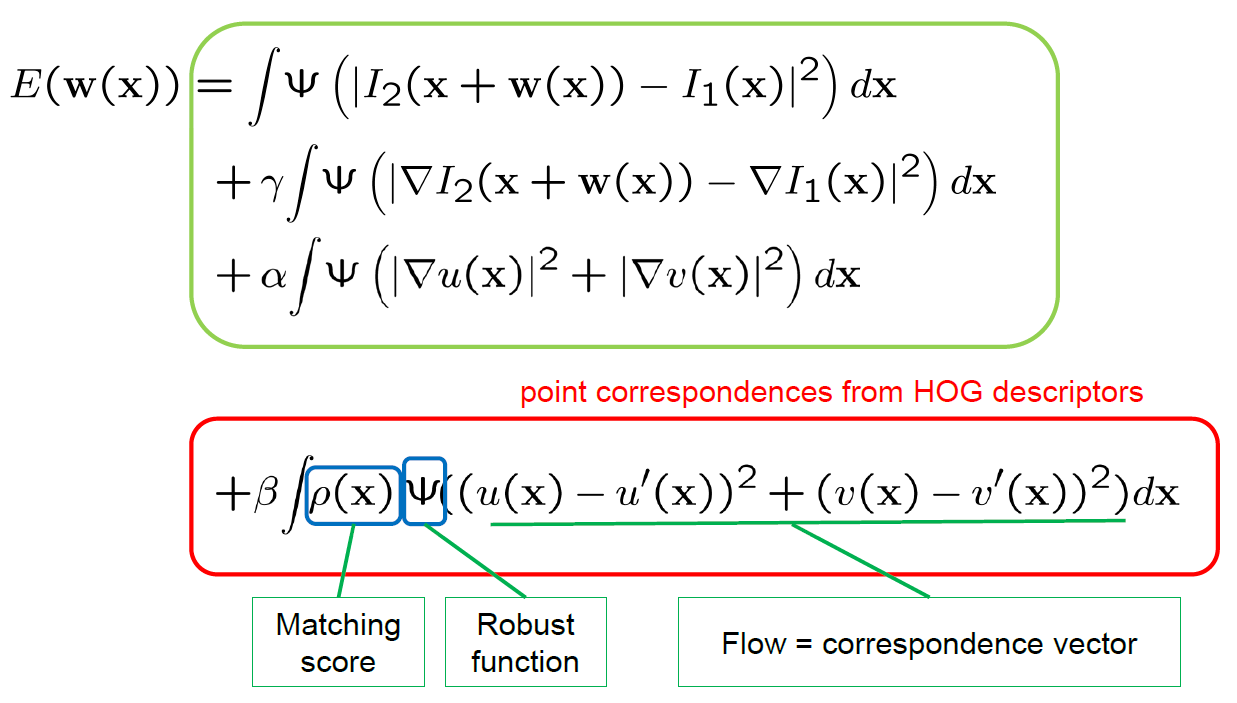
\includegraphics[width=0.6\textwidth]{flow.png}
\end{figure}

\b{Coarsed-to-fine effect:} At the beginning (low-res) you have a high number of nearest neighbor matches (computed at high-res) compared to the number of pixels. By improving the resolution the outlier matches are removed step-by-step.

\subsection{Optical Flow with a Deep Network}
\begin{itemize}
    \item Two images at input. Encoder who analyses that information
    \item Decoder produces optical flow field at the original resolution
    \item Problem: Where to get the data and ground truth optical flow field? \f{\to} Synthetic data
    \item \b{FlowNetC:} Two input CNNs learn features that are good to match. These features then get correlated in a special correlation layer, which produces a cost volume with the result of the correlation. The decoder can then analyze the cost volume and produce optical flow.
    \item \b{FlowNet2:} Improved data and training schedules, stacking of networks with motion comp.
    \item \b{FlowNet3:} Residual connections across networks
    \item \b{Advantage:} As accurate as best classical methods but much faster.
    \item \b{PWC-Net:}
    \begin{itemize}
        \item Start with downsampled images, compute energy minimization and get initial flowfield that you upsample for the next iteration.
        \item Take the next upsampling resolution and do the same and take the upsampled flow field as initial one for the energy      minimization.
        \item Repeat until you are at the original resolution and get the final resulting flow field.
    \end{itemize}
    \item \b{RAFT:}
    \begin{itemize}
        \item Multi-scale cost volume (robust matching at cost volume level)
        \item Context encoder (improves sharp boundaries)
        \item Recurrent architecture for refinement
    \end{itemize}
    \item \b{Note:} Generalization properties are much better than for recognition networks!
\end{itemize}

\newpage
\section{Video Segmentation}
The issue with video segmentation is to find the object regions for learning. Color and texture might work in some special cases but usually does not. Instead we can find (moving) object regions by motion segmentation. 

\subsection{Motion Segmentation}
The goal of motion segmentation is to separate regions by their motion. The problem is that the computation of motion is error-prone and not unique in all areas. This leads to a two-variable problem: We need to estimate both motion field and partitioning, but need one to estimate the other. The standard approach to get around this is to:
\begin{enumerate}
    \item First compute optical flow
    \item Then compute segmentation based on optical flow
\end{enumerate}
\b{Problem:} Object flow requires distinct object motion in all frames of interest.\\

\b{Motion Segmentation based on Point Trajectories:\\[0.5em]}
Two-frame optical flow can only separate objects with different motion in these two particular frames. The idea to circumvent this is to make use of the temporal context of the frames and use \b{point trajectories over multiple frames}. These trajectories can be obtained via point tracking (concatenation of optical flow vectors). Clustering based on the full trajectories can separate objects even when they don't move.\\

One issue is that trajectories have different lengths (mostly due to occlusion/disocclusion). Can be solved by:
\begin{enumerate}
    \item Establish distances for all pairs that share common frames
    \item Transitivity in the graph can connect pairs even if they do not share common frames (if a trajectory stops and reappears and another trajectory has the same motion, they are connected and put into the same cluster.)
    \item Assumption: Points that move together belong together (Gestalt law)\\
    \f{\to} For each pair consider the maximum motion difference over time \f{d(a,b)=\max_td_t(a,b)}
\end{enumerate}

In own words: We have multiple frames and concatenate the flow vectors of each frame for each pixel. Then we apply spectral clustering by comparing the trajectories.\\

\b{Note:} A difficulty is if something moves towards the camera (scaling motion instead of translation, density of grid would increase).\\

\b{Dense Estimation:\\[0.5em]}
So far we only looked at sparse estimation, but we usually want dense estimations (e.g. segmentation map). With given sparse labels it would not be hard to train a model to produce the dense labels (requires training data). There are, however, variational label interpolations as well.

\subsection{Video Tracking}
An alternative to motion segmentation, which yield multiple objects and can be realized with modern encoder-decoder networks (simplifies the problem). Requires segmentation in the first frame.
\newpage
\section{3D Geometry and Camera Calibration}
\subsection{Basics}
\b{Pinhole Camera:} The most popular projection model, even though it neglects the effect of lenses. In this model, a 3D point \f{X = \top{(X,Y,Z)}} is projected onto a point in the image plain via:
\cf{x = f\frac{X}{Z}\quad,\quad y=f\frac{Y}{Z}}
This projection is nonlinear due to the division by \f{Z}, meaning the height in the image plane is not linear to the real height \f{Z}.\\
To avoid this nonlinearity in calculations, we can work in so-called homogenous coordinates by adding a 1 to the end of the coordinate vector:
\cf{
    (x,y)\in\mathbb{R}^2\quad\to\quad(x,y,1)\in\mathbb{P}^2
}
To get back to Euclidian space we simply have to divide by the third coordinate.\\

Using homogenous coordinates, the projection from above becomes linear (only when recalculating the Euclidian coordinates we have to divide):
\cf{
    \begin{pmatrix}
        x' \\
        y' \\
        z' 
    \end{pmatrix} =  
    \begin{pmatrix}
        f & 0 & 0 & 0 \\
        0 & f & 0 & 0 \\
        0 & 0 & 1 & 0 
    \end{pmatrix} \begin{pmatrix}
        X \\
        Y \\
        Z \\
        1 
        \end{pmatrix}
}
\cf{
    x=\frac{x'}{z'}\quad,\quad y=\frac{y'}{z'}
}
The linear operator \f{P} is called \b{projection matrix} with \f{x=PX}. So far the matrix has many zero entries. In general, all 12 entries are different from zero describing a general projective camera. However, the matrix has only 11 degrees of freedom because scaling does not change the resulting 2D point (in Euclidean coordinates).\\
The task to determine the entries of the projection matrix is called \b{camera calibration}. Knowing the projection matrices of the involved cameras is required for 3D point reconstruction from 2D point correspondences. \\

The projection matrix can be factorized into two parts \f{P=KM}, where:
\cf{K=\begin{pmatrix}
    \alpha_x & s & x_0 \\
    0 & \alpha_y & y_0 \\
    0 & 0 & 1 
    \end{pmatrix}}
is the \b{camera calibration matrix} containing the camera's internal parameters. The second part, \f{M=(R|t)}, is the pose of the camera relative to a world coordinate system. \f{M} consists of a rotation matrix \f{R} and a translation vector \f{t}, each having 3 degrees of freedom. These are the external parameters.\\

\b{Note:} \f{P} must have rank 3 to project to a plane.\\

\b{Meaning of the parameters of K:}
\begin{itemize}
    \item \f{\alpha_x}: focal length times pixel width in x-direction
    \item \f{\alpha_y}: focal length times pixel width in y-direction
    \item \f{x_0,y_0}: origin in the image plane (principal point)
    \item \f{s=\alpha_x\cos\phi}: skew parameter (almost always 0)
\end{itemize}
\newpage
\b{Note:} if \f{\alpha_x=\alpha_y} then the pixels are square and the number of free parameters decreases. The other parameters vary from camera to camera and must be determined by a calibration procedure. The focal length may even change while recording a video, e.g. because of autofocus.\\

\b{Affine projection / camera model:}
The \b{affine projection} is an approximation of the perspective projection that leads to linear mappings also in Euclidean coordinates. The \b{affine camera model} only has 8 free parameters:
\cf{
    P = \begin{pmatrix}
        m_{11} & m_{12} & m_{13} & t_1 \\
        m_{21} & m_{22} & m_{23} & t_2 \\
        0 & 0 & 0 & 1 
        \end{pmatrix}
}
\b{Note:} This camera model is (only) a good approximation if objects are far from the camera and have a small variation in depth.


\subsection{Camera Calibration}
Camera calibration denotes the process that estimates the camera parameters from suitable images. \b{Full calibration} yields the projection matrices of all involved cameras in a common world coordinate system. For this we need information about the true size of the observed object and its pose in the world coordinate system. Sometimes this is not available, e.g., in structure from motion. In this case the calibration procedure shall determine the camera's internal parameters.\\

\b{Full Camera Calibration from 2D-3D Correspondences:\\[0.5em]}
The classical procedure is based on a \b{calibration object} with known 3D points (e.g. black squares image). Observation of these points in the image yields 2D-3D correspondences.\\
In the example of the image with the black squares, the 2D point correspondences could be found by a corner detector. This works by applying an edge detector, then fitting lines to the edges (Hough transform) and finding the crossings of the lines.\\
From the retrieved point pairs \f{x_i,X_i} we can estimate the camera parameters. Each point correspondence has the constraint:
\cf{x_i\times PX_i = 0}
Since we are in homogenous coordinates, two points are equivalent if their vectors have the same direction, which is expressed by the cross product.\\

\begin{figure}[h!]
    \centering
    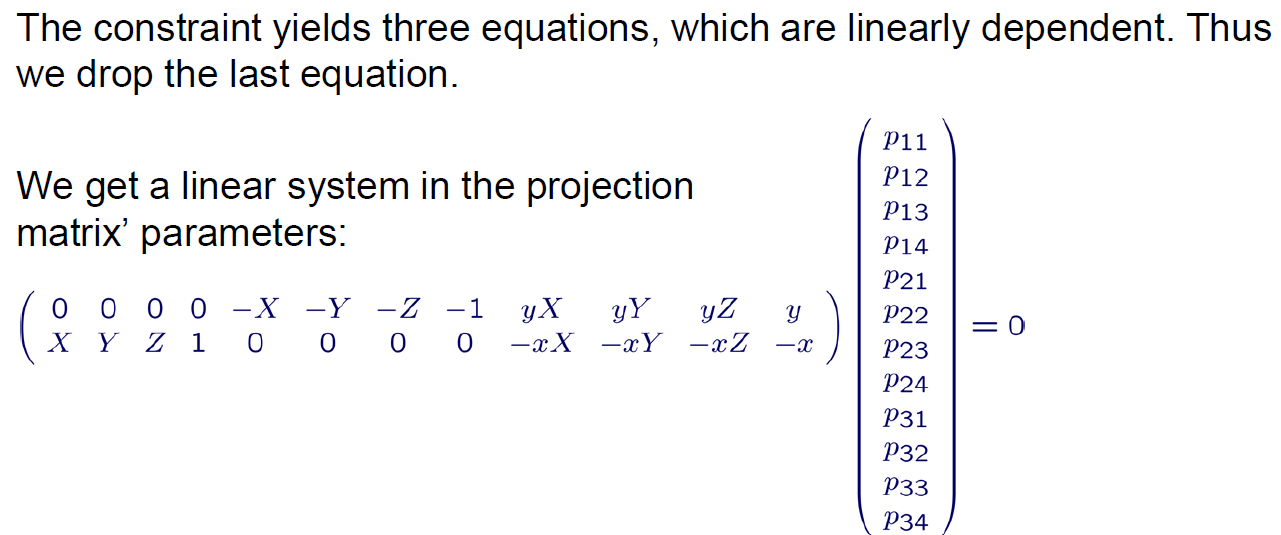
\includegraphics[width=0.6\textwidth]{cali.png}
\end{figure}

For each point correspondence we get such a system and by stacking the equations we get a system with \f{2N\times 12} \b{system matrix} \f{A}. We need at least 6 point correspondences. All we have to do is solve (minimize) the over-determined system \f{Ap=0} while avoiding the trivial solution \f{p=0}.\\
Note that we have 12 parameters but only 11 degrees of freedom. The best way is to introduce the constraint \f{||p||=1}. Then we end up with the minimization problem of \f{\frac{||Ap||}{||p||}}. This can be achieved by SVD (quite complex to compute). The solution is just the singular vector corresponding to the smallest singular value (not \it{eigen}, since A is not quadratic).
\newpage
\b{Normalization:\\[0.5em]}
The accuracy of the calibration matrix depends on the accuracy of the extracted corner points in the image. For accurate estimates it is important that the errors are treated homogeneously. This can be achieved by normalizing the 3D points as well as the 2D points such that their centroids are at 0 and the average distance of points to the centroid is \f{\sqrt{3}} and \f{\sqrt{2}} respectively.\\
The transformations to do so (shift and scaling) are expressed by matrices \f{U} and \f{T}. We then estimate the projection matrix \f{\tilde{P}} with the transformed points and retrieve \f{P} by \f{P=T^{-1}\tilde{P}U}.\\

\b{Note:} Up to this point the procedure only works if the calibration object (the 3D points) is \b{coplanar}. This requires a calibration object of at least two planes (precise measurement rather difficult).\\

\b{Note:} An alternative calibration method would be from multiple views of the same \it{planar} calibration object. Except for multi-camera setups this is much more convenient.

\subsection{General Projection to Homography}
In general, the projection is described as follows:
\cf{
    \begin{pmatrix}
    x \\
    y \\
    1 
\end{pmatrix} = K\cdot
\begin{pmatrix}
    r_1 & r_2 & r_3 & t
\end{pmatrix}
\begin{pmatrix}
    X \\
    Y \\
    Z \\
    1 
    \end{pmatrix}}
But now that all points lie in a plane, we can, without loss of generality, choose the world coordinate system such that this plane is \f{Z=0}:
\cf{
\begin{pmatrix}
    x \\
    y \\
    1 
\end{pmatrix} = K\cdot
\begin{pmatrix}
    r_1 & r_2 & r_3 & t
\end{pmatrix}
\begin{pmatrix}
    X \\
    Y \\
    0 \\
    1 
\end{pmatrix} = K\cdot
\begin{pmatrix}
        r_1 & r_2 & t
    \end{pmatrix}
\begin{pmatrix}
        X \\
        Y \\
        1 
\end{pmatrix}
}
The projection is a plane to plane mapping involving only 2D coordinates. Such a mapping is described by a homography (\f{x' = Hx}), which can be estimated by 2D point correspondences.\\

Homography estimation works the same way as estimation of the projection matrix discussed before. \f{H} is even a projection in a simplified setting (all points lying in a plane). With the constraint that all corresponding points must have the same direction
(\f{x'\times Hx = 0}), 
we can obtain three linear dependent equations from each point correspondence (we only keep two):
\cf{
    \begin{pmatrix}
        0&0&0-x&-y&-1&y'x&y'y&y'\\
        x&y&1&0&0&0&-x'x&-x'y&-x'
    \end{pmatrix}h=0
} 
Considering \f{n} correspondences we get a linear system \f{Ah=0} with \f{A\in\mathbb{R}^{2n\times 9}}, subject to \f{||h||=1}. The solution can again be obtained by SVD. To treat errors in the correspondences homogeneously the points should again be normalized. This can be done by applying a normalizing transformation \f{T} to all points \f{x_i} such that the centroid is in the origin and the average distance to the origin is \f{\sqrt{2}}.\\

\b{Homography decomposition:\\[0.5em]}
The estimated homographycontains the internal and external camera parameters:
\cf{H=K\cdot(r_1\ r_2\ t) \qquad (h_1\ h_2\ h_3) = \lambda K\cdot(r_1\ r_2\ t)}
From this, we can derive two constraints for decomposition: (1) \f{r_1} and \f{r_2} must be orthogonal, (2) the rotation vector itself should be 1.
\newpage

Since we have two equations (restraints) for 5 unknowns, either three of the internal camera parameters need to be known or we need additional constrains from further homographies! These homographies are obtained by moving the camera (or the plane). The motion must comprise a rotation and the internal parameters must not change. At least 3 views are needed to estimate all 5 parameters. Once the internal parameters are known, the external parameters for each view can be estimated.\\

\b{Left out: Mathematical decomposition process}\\

\b{Note:} Due to estimation errors, the rotation matrix is usually not a proper rotation matrix with \f{R^\top R=1}. This can be enforced by applying an SVD \f{R=UDV^\top}.

\subsection{Radial Distortion}
With the pinhole camera model the projection was a linear operation in homogenous coordinates. However, the pinhole camera neglects the effect of lenses, which have a nonlinear effect on the projection (can not be described by projection matrix). This effect becomes increasingly relevant for decreasing focal length (e.g. fisheye effect). The distortion can be modeled as:
\cf{
    \begin{pmatrix}
        x\\
        y
    \end{pmatrix} = L(r)
    \begin{pmatrix}
        \tilde{x}\\
        \tilde{y}
    \end{pmatrix}
}
where \f{L(r)} is a function that depends only on the distance of a point to the center of distortion (usually the principal point \f{(x_0,y_0)} of the camera). \f{L(r)} can be modeled as:
\cf{
    L(r) = 1+\kappa_1r+\kappa_2r^2+\kappa_3r^3+...
}
The coefficients can be estimated from the correspondences by minimizing a cost function that penalizes the deviation from the linear mapping in the calibration procedure:
\begin{itemize}
    \item Calculate ideal distortion free projected points \f{(\tilde{x}, \tilde{y})} with \f{P}
    \item Calculate distance \f{r=\sqrt{(\tilde{x}-x_0)^2+(\tilde{y}-y_0)^2}} from principal point to projected points
    \item Observe/measure the actual image point (not the projected one)
    \item Calculate coefficients of \f{L(r)} to compensate displacement of points
\end{itemize}

\newpage
\section{Stereo Reconstruction}
Stereo reconstruction is a powerful way to reconstruct depth of scenes by point correspondences between different views of the scene. There are multiple steps to stereo reconstruction:
\begin{enumerate}
    \item Calibration and estimation of the epipolar geometry (correspondences must lie on a line)
    \item Disparity estimation to find the correspondences
    \item Triangulation: Reconstructing the 3D point from 2D correspondences
\end{enumerate}

\subsection{Epipolar Geometry}
The epipolar geometry is independent of the scene structure. It depends only on the internal camera parameters and their \b{relative} pose.\\
The corresponding point in the other camera must lie on the projected projection ray (epipolar line):

\begin{figure}[h!]
    \centering
    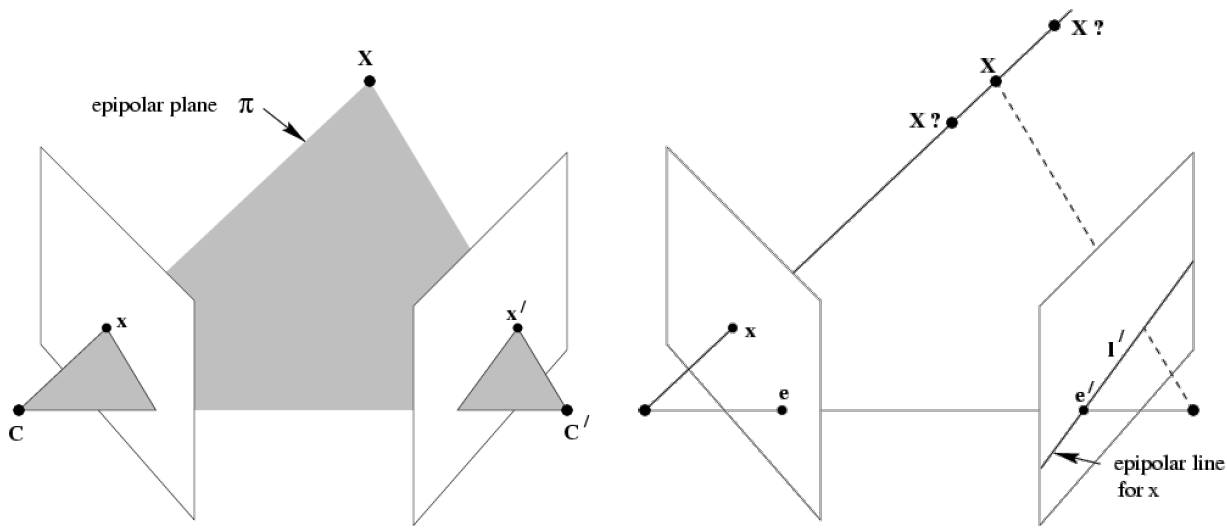
\includegraphics[width=.8\textwidth]{line.png}
\end{figure}

The projection ray itself can be constructed using the camera parameters. The projection of the camera center in the other camera \f{C} is called \b{epipole} \f{\pmb{e}}. All epipolar lines go through the epipole. If it is visible in the image, it is also called \b{focus of expansion}.\\

\b{Fundamental Matrix:\\[0.5em]}
The epipolar geometry is fully described by the so-called fundamental matrix \f{F^{3\times3}} (rank 2). It describes the mapping of an image point in one camera to the corresponding epipolarline in the other camera (homogenous coordinates):
\cf{
    l' = Fx \qquad,\qquad l=F^\top x'\qquad,\qquad x'^\top Fx=0
}
\b{Note:} \f{F} can be estimated from 2D correspondences alone (in contrast to \f{P}).\\

If we know the projection matrices of two cameras, the fundamental matrix can be derived as:
\cf{
    F = [e']_\times P'P^\dagger ,
}
where \f{e'} is the epipole in the second camera with \f{e'=P'C}. \f{C} is obtained by solving \f{PC=0}. \f{P^\dagger} is the pseudo-inverse of \f{P} with \f{P^\dagger :=(P^\top P)^{-1}P^\top}. \f{[e']_\times} denotes the skew-matrix (not included).\\

If we have point correspondences, we can estimate the fundamental matrix without the need of a calibrated camera. Due to the line-constraint from above and the rank-2 constraint, it has 7 degrees of freedom. However, it is easier to over-parametrization with 9 parameters and a constraint on the scale, which leads to the \b{8-point algorithm} (similar to calibration/homography).
\newpage

Here, normalization is even more important, as \f{F} is more sensitive to noise in the correspondences because the pixel positions will be squared (so the error will be squared too).\\
Combining the constraints from \f{N} correspondences we get the linear system \f{Af=0} with \f{A\in\mathbb{R}^{N\times 9}}. The solution is obtained as the singular vector to the smallest singular value of \f{A}.\\ This estimate does usually not satisfy the rank constraint, which can be enforced afterwards by and SVD of \f{F}, setting the smallest singular value to 0.\\

Higher accuracy estimates are obtained by iterative procedures that start with the 8-point algorithm for initialization and then refine the estimate. Iteration is necessary since the distance measures are nonlinear.\\

\b{Reprojection Error:} The F-matrix is estimated together with the reconstructed 3D points. The error between the reprojected 3D points and the 2D points is minimized (bundle adjustment).\\

\b{Outliers:\\[0.5em]}
Estimation methods as introduced can deal with small (Gaussian) errors. However, calculating correspondences can yield a few false matches (e.g. because of occlusion), so called \b{outliers}. These outliers can severely disturb the results, which is why they have to be removed.\\

\b{Random Sample Consensus (RANSAC)} is a method for outlier identification and estimating parameters only from inliers:
\begin{enumerate}
    \item Randomly select subset of mimimum size
    \item Estimate model from this subset
    \item Determine the number of points that are consistent with this model (number of inliers, \b{support})
    \item Repeat these steps with different subsets and choose subset with largest support
    \item Estimate model from all inliers
\end{enumerate}

In practice: You collect 200 point corr. for the image pair. Now you sample 8 random correspondences of the 200, put them into the 8-point-algorithm and get an estimated F-matrix (model). Next you check how good the remaining 192 points fit into the new F-matrix. Choose a treshild and estimate which correspondences are inliers and which are outliers. Repeat the previous steps with different subsets and choose the F-matrix with the most inliers. Then estimate the F-matrix from all these inliers.\\

\b{Note:} The chance of picking a subset consisting only of inlier increases with the number of iterations. It decreases with the size of the subsets (degrees of freedom).\\

\b{Autocalibration:\\[0.5em]}
The F-matrix can be estimated without the need of a calibration tool. This means you can simply take two pictures from different views of an object and perform the calibration with them.\\
The idea: Given the F-matrix we can derive a canonical form of the P-matrices (autocalibration via F-matrix):
\cf{
    P=(I|0)\qquad P'=([e']_\times F|e')\qquad 
}
where \f{e'} is obtained by solving \f{F^\top e'=0}. The first projection matrix (\f{P}) is set as the identity with zero vector to fix the world coordinate system.\\
\b{Problem:} Many other projection matrices satisfy the constraints given by the F-matrix (both P-matrices have a combined total of 22 degrees of freedom, while the F-matrix only has 7). The remaining 15 degrees of freedom describe a 3D projective transformation (which should only have \f{3\times 3}), which leads to \b{projective amiguity}. \f{\to} Metric reconstrucion

\subsection{Metric Reconstruction}
For a metric reconstruction only the internal camera parameters must be known. This fixes 10 of 15 degrees of freedom. We can then derive the relative pose of the two cameras, known as \b{egomotion}, up to a scale factor. Knowing that we can compute the normalized coordinates of the image points as:
\cf{
    \hat{x} = K^{-1}x\qquad,\qquad \hat{x}' = K'^{-1}x'
}
From point correspondences we can estimate the \b{essential matrix} \f{\pmb{E}} with \f{\hat{x}'E\hat{x}=0}. \f{E} is related to \f{F} and the egomotion via:
\cf{
    E=K'^\top FK = [t]_\times R = R[R^\top t]_\times
}
The essential matrix only has 5 d.o.f, while the F-matrix has 7. This means that one can derive \f{E} directly (when knowing the camera parameters). However, \f{E} can also be estimated with the 8-point algorithm enforcing the constraints of rank 2 and the first two singular values being one.\\
Because \f{E} is related to the egomotion, we want to calculate the positions of camera in the images. For that we can decompose \f{E} via SVD into \f{E=U\text{diag}(1,1,0)V^\top} and fix \f{P=(I|0)} for the first image. Due to sign ambiguity of SVD this results in for possible positions (rotations and translations) of the camera in image two, of which only one solution can be true (verification: a single point must be in front of both cameras).\\

Even though metric reconstruction removes the projective ambiguity of autocalibration, there are still some similarity ambiguities left (translation, rotation, scaling). For example: Is an object big and far away or close and small? These ambiguities can partly be answered by landmarks and objects of known size in the scene. The scale amiguity can also be avoided through fixed stereo cameras.

\subsection{Triangulation}
With given correspondences and P-matrices we can traingulate the 3D points. For perfect measurements the following restraints hold:
\cf{
    x=PX\qquad,\qquad x'P'X
}
However, often the image points do not satisfy the epipolar constraint exactly (projection rays miss each other). The solution can be found in the least squares sense.\\

The direction of the projected 3D points must coincide with the image points:
\cf{
    x\times (PX) = 0\qquad,\qquad x'\times (P'X) = 0
}
This results in three constraints for each of the two points, of which two are linearly independent. By combining the restraints we get the linear system \f{AX=0} with \f{A\in\mathbb{R}^{4\times1}}.\\
For projective reconstruction the constraint \f{||X||=1} is added. For metric reconstruction the \f{4^{\text{th}}} \f{X}-component is fixed: \f{X=(X,Y,Z,1)^\top}.\\

\b{Uncertainty in the estimate:\\[0.5em]}
The uncertainty in the exact position of the corresponding point in the other image propagates to the depth estimate. The propagation is more severe the more parallel two rays are.\\
Hence, a large baseline is positive for accurate depth measurements, but it also makes finding corresponding points harder (larger search range, more distortion, more occlusions).
\newpage
\section{Disparity Estimation and Scene Flow}
Disparity is the signed distance between images of the same 3D point in two views. Thus it is a special case of optical flow.\\

\b{Comparison to optical flow:}
\begin{itemize}
    \item Disparity is a scalar function rather than a vector field due to the epipolar constraint (1D-Problem)
    \item Makes optimization much easier
    \item Usually we want much larger displacements (more accurate depth)
    \begin{itemize}
        \item Local optimization becomes problematic
        \item Occlusion is more relevant
    \end{itemize}
    \item Disparity estimation has been dominated by combinatorial techniques, now by deep networks
\end{itemize}

\b{Goal/Idea:} Search in both pictures for corresponding points to calculate the difference. It would be easier to find the pixel in second image if we only had to search in one row \f{\to} Transformation of image(s) to have parallel epipolar lines.\\

\b{Special stereo setting:} Using a stereo camera, the camera motion is (approx.) a translation parallel to the x-Axis. Thus the epipolar lines are the image rows.

\subsection{Rectification}
\b{Goal:} Turn a general camera setting into special case with epipolar lines being horizontal scan lines. Can be done by mapping the individual image planes to a plane parallel to the baseline: \f{x'=Hx} (described by homography). Note that the homography shifts the epipoles to infinity. In case the epipole is visible in the image, a polar representation is needed (changes size/dimensions of points but makes epipolar lines parallel).\\

\b{Estimation of rectifying homography:\\[0.5em]}
Given the F-matrix \f{F} we want to find out the rectifying homography \f{H}:
\begin{enumerate}
    \item Get the epipole \f{e'} from \f{F} by solving \f{e'^\top F=0}.
    \item Find out transformation that maps epipole to \f{e'=(1,0,0)^\top}: \f{He'=(1,0,0)^\top}
    \begin{itemize}
        \item Leaves 5 degrees of freedom
        \item Additional constraint: minimize distortion around a point of interest \f{x_0}
    \end{itemize}
    \item Optional: Take both image planes into account, choose a new plane to map to, calculate and minimize the average distortion of both images (requires point correspondences6)
\end{enumerate}

\subsection{Overview of Methods}
\b{Variational methods:}
\begin{itemize}
    \item Removing the v-component from optical flow methods (rectified)
    \item Optimization for non-rectified images possible
    \item Local optimization suboptimal due to large displacements
\end{itemize}
\newpage
\b{Combinatorial optimization:}
\begin{itemize}
    \item Line-wise message passing (rectified)
    \item Semi-global matching
\end{itemize}
\b{Deep Learning:} DispNet (special case of FlowNet)

\subsection{Variational Methods for non-rectified Images}
As the images are not rectified, we need to include the epipolar constraint in the optical flow method.\\
The epipolar line is usually defined as:
\cf{
    l'(x) = Fx =: \begin{pmatrix}
        a(x)\\b(x)\\c(x)
    \end{pmatrix}
}
Then the optical flow vector \f{w:=(u,v)^\top} can be expressed through the disparity \f{d(x)} along the epipolar line \f{l'(x)}. With this the optical flow energy functional can be modified to:
\cf{
    E(d)=\int_\Omega\Psi\left((I_2(x+w(d)))-I_1(x)^2\right)+\alpha\Psi\left(|\nabla d|^2\right)dx
}
\b{Advantage:} Subpixel accuracy. However, results are not convincing.

\subsection{Similarity Measures}
The requirements are similar to optical flow estimation, such as:
\begin{itemize}
    \item Robustness to illumination changes is important
    \item Matching only small patches (ideally pixels) or learned features to ensure high accuracy
\end{itemize}

However, there are some differences too:
\begin{itemize}
    \item Appearance changes are only due to viewpoint, no temporal effects
    \item Global illumination changes are rare
    \item Mostly local reflectance changes due to non-Lambertian surfaces
    \item Occlusion areas tend to be much larger
    \item Occlusion can be derived from the disparity estimate
\end{itemize}

The sum of squared differences compares the color of two batches in the left and right image and is thus sensitive to different reflectance. \f{\to} Use gradient instead of color.\\

\b{Normalized cross correlation} is a similarity measure that is invariant to additive and multiplicative intensity changes. The results are in the range \f{[-1;1]}, where -1 stands for anti-correlation and 1 stands for correlation. To avoid problems in areas without structure, a small constant is added to the denominator. This leads to homogeneous patches having 0 correlation.

\subsection{Combinatorial Optimization}
Combinatorial optimization has been the standard for disparity estimation before being replaced by DL.\\

\b{Message Passing\\[.5em]}
In general the energy on a graph with nodes \f{p}, neigboring nodes \f{q}, pixel labels \f{x\in\{1,...,L\}} and cost \f{\theta} is given by:
\cf{
    E(x) = \sum_p\theta(x_p)+\sum_{p,q\in\mathcal{N}(p)}\theta_{pq}(x_p,x_q)
}
For disparity estimation the labels \f{x} correspond to the disparities, the unary cost \f{\theta(x_p)} is the matching cost and the pairwise cost \f{\theta_{pq}} is a smoothness constraint (neigbors should have similar disparities).\\
If the graph is a tree, a global optimimum can be found by message passing via a forward and backward sweep.\\

The problem can be simplified by estimating the disparity in each image row independently:
\begin{itemize}
    \item Smoothness only in x-direction
    \item Graph in each row is a chain (tree) \f{\to} message passing applicable
    \item Drawback: No smoothness in y-direction
\end{itemize}
\vspace{0.5em}
\b{Semi-Global Matching (SGM)\\[.5em]}
SGM extends the previous approach by considering lines in multiple directions, where each line is still a message passing problem on a chain. For each pixel, the messages from all directions have to be considered.\\

\b{Note:} This is not globally optimal (loops are ignored), but a good approximation.\\

SGM consists of two parts:
\begin{itemize}
    \item Matching costs
    \item Optimization along scan lines
\end{itemize}

\subsection{Deep Networks for Disparity}
\b{SGM with Cost from Deep Network\\[.5em]}
The matching cost for the SGM method can be computed with a siamese network (two heads), which was trained on matching and non-matching patches. Thee network then learns the feature representations of the patches and the metric to compare them.\\

\b{Advantage:} Removes the need for choosing a (suboptimal) metric.\\
\b{Drawback:} One full network pass is needed for each patch comparison.\\

\b{Disparity Networks:\\[.5em]}
Very similar to the original FlowNet structure, can compute the full disparity map at once. The correlation layer inside the network yield a cost volume. The rest of the network then interprets the result of the cost volume.
\newpage
Advantages:
\begin{itemize}
    \item Interactive frame rates on the GPU
    \item Exploits global context between the images (no patch sizes involved)
    \item Outputs are real numbers: no accuracy limit due to quantization
    \item The networks learns how to deal with ambiguities
\end{itemize}

\subsection{Scene Flow}
Scene flow (for videos!) includes depth estimation, optical flow estimation, and estimation of the change in depth. \f{\to} Yields 3D point and its 3D motion vector.\\

Scene flow can be optimized just as optical flow, but this comes with the downside of being supoptimal for stereo. 
Instead, we can separate the depth estimation by applying SGM, which is also applicable directly to RGB-D videos.\\

Deep Networks for scene flow are a combination of FlowNets and DispNets.
\vspace{2cm}
\begin{figure}[h!]
    \centering
    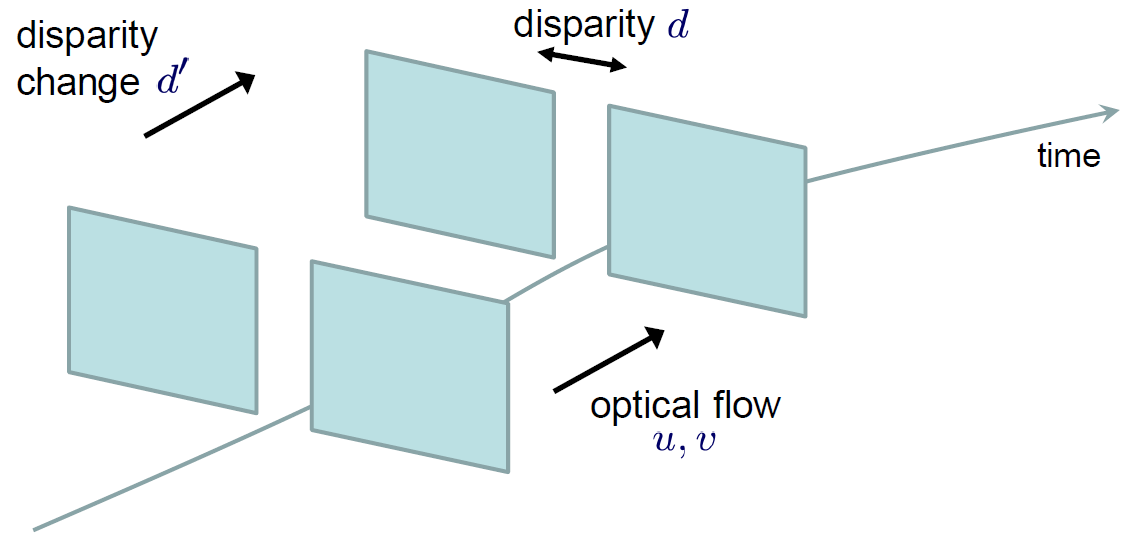
\includegraphics[width=.6\textwidth]{scene.png}
\end{figure}

\newpage
\section{Structure from Motion}
\b{Given:} Stereo case extended to more than two cameras by either adding more cameras or moving the same camera in space.\\

\b{Goal:} Estimate camera position AND 3D reconstruction of the scene.\\

\b{Important:} We observe a \b{static} scene from multiple viewpoints \b{over time}.\\

The F-matrix counterpart in the three-point case is called the \b{trifocal tensor} (also available in four-camera case \f{\to} quadrifocal) and describes the constraints for corresponding points in three (or four) cameras. This tensor representation stops for more than four views and we need to handle it differently.\\


\subsection{Overview}
\begin{itemize}
    \item Given the internal camera parameters, the essential matrix \f{E} can be estimated from 2D point correspondences of the camera motion.
    \item Internal camera parameters and essential matrix are sufficient for metric reconstruction.
\end{itemize}
For structure from motion we need:
\begin{itemize}
    \item Internal camera parameters
    \item Sparse point correspondences to estimate \f{E}
    \item Sparse or dense point correspondences to reconstruct scene
    \item An optimization process to couple these processes to refine the result (\f{\to} Bundle Adjustment)
\end{itemize}

\subsection{Bundle Adjustment}
In the general case, we want to optimize the projection matrices \f{P^i} of all cameras and all 3D points \f{X_j} given the image points \f{x_j^i} by minimizing the reprojection error:
\cf{
    \min_{P^i, X_j}\sum_{ij}d^2(P^iX_j, x_j^i)
}
\begin{figure}[h!]
    \centering
    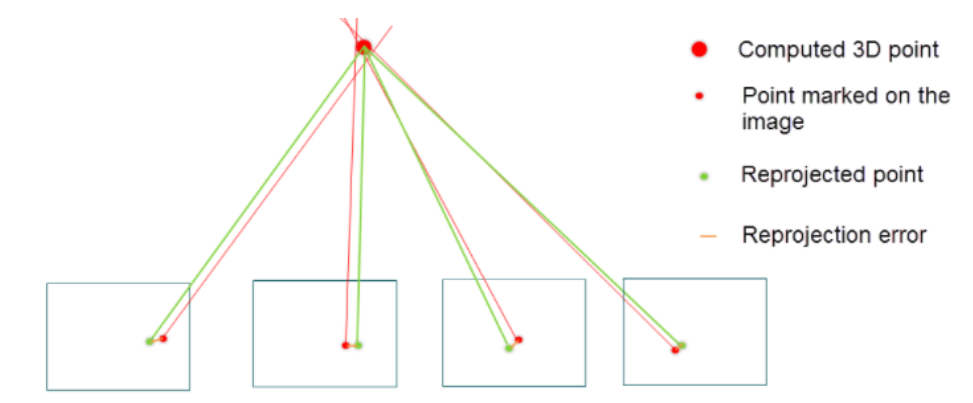
\includegraphics[width=0.5\textwidth]{bundle.png}
\end{figure}

Note that this general case is very sensitive to noise. Knowing the internal camera parameters of each camera, only their rotation \f{R^i} and translation \f{t^i} relative to a reference need to be estimated, which leaves us with:
\cf{
    \min_{R^i, t^i, X_j}\sum_{ij}d^2(P^i(R^i, t^i)X_j, x_j^i)
}
The intuition here is that we need to shift and rotate the bundle of projection rays such that the point distances \f{d(x,y)} get minimized.\\

\b{Advantage:} Bundle adjustment is very flexible with regard to the model. We can even estimate some internal camera parameters by adding them to the term and adding a prior.\\
\b{Drawback:} The cost function is nonlinear and non-convex with many local minima. So we need to get good initialization and then refine using bundle adjustment.\\

\b{Linear BA with Factorization Algorithm\\[.5em]}
The linear bundle adjustment method is based on the affine camera model with 
\cf{
    P=\begin{pmatrix}
        m_{11}&m_{12}&m_{13}&t_1\\
        m_{21}&m_{22}&m_{23}&t_2\\
        0&0&0&1\\
    \end{pmatrix} \quad\to\quad
    \begin{pmatrix}
        x\\y
    \end{pmatrix} = M
    \begin{pmatrix}
        X\\Y\\Z
    \end{pmatrix} + t
}
by which the projection becomes linear. This approach, however, assumes that the depth variation in the scene is small compared to the distance to the camera. In the linear case the reprojection error becomes a simpler problem:
\cf{
    E(M^i, t^i, X_j) = \sum_{ij}||x_j^i-(M^iX_j + t^i)||^2\quad,
}
which leads to \f{t_i = \mu_i = \frac{1}{n}\sum_jx_j^i}. Subtracting the centroid \f{\mu^i} from the sum leads to \f{t^i = 0}, by which the remaining optimization problem becomes a factorization problem:
\cf{
    E(M^i, X_j) = \sum_{ij}||x_j^i-M^iX_j||^2
}
The problem with this factorization method is that it requires creating the measurement matrix \f{W} from all points \f{x_j^i}, so all points must be visible in all cameras, which is bad for large scenes! Using SVD this measurement matrix is the factorized.\\
The solution then however still contains the scale ambiguity of metric reconstruction and the affine ambiguity (\f{W=MAA^{-1}X} for any rank 3 matrix \f{A}). The remove the affine ambiguity we can use metric reconstruction with the internal parameters to compute the position of the camera.\\

\b{Initialization of BA\\[.5em]}
Factorization could provide an initialization for subsets of images where all points are visible in all frames, which is typically unrealistic.\\
More common is to use the minimum subset of two images (where all points are visible) and then add more views incrementally.\\

With only two frames the process is similar to previous chapters: Estimate the essential matrix from point correspondences and factorize it into relative translation and rotation.\\
Then, using transitivity, if we know the motion from frame A to frame B and from B to C, we can get the motion from A to C:
\cf{
    R_{AC} = R_{BC}R_{AB}\qquad,\qquad t_{AC} = R_{BC}t_{AB}+t_{BC}
}

\b{Initial reconstruction:}
\begin{enumerate}
    \item Build projection matrices \f{P^i = K^i(R^it^i)}
    \item Triangulate 3D points \f{X_j} from projection matrices and 2D points
    \item Use constraints from all cameras where point \f{X_j} is visible to solve \f{AX_j=0}
\end{enumerate}
\newpage
\b{Incremental BA\\[.5em]}
If we initialize bundle adjustment well enough and there are points jointly visible in distant images, bundle adjustment is a global optimization that optimally corrects drift (accumulation of errors).\\

To mitigate drift, we can run bundle adjustment after adding a new frame to the chain. Note that this is rather slow and can not run in realtime. \b{Loop-closing} also reduces drift by adding long-distance correspondences but also adds risk of adding more drift in some cases.\\

\b{Optimization\\[.5em]}
With a good initialization, the solution can be refined by minimizing the highly nonlinear reprojection error (from before). The nonlinearity is due to the distance \f{d(x,y)} in image coordinates, which requires division by the third component.\\
Due to outliers, it further makes sense to use a robust norm \f{\Psi(d)}, which would add another nonlinearity.\\
This problem can then be minimized via the \b{Levenberg-Marquardt} method (or Gauss-Newton, but that's not always stable in BA). \\

The Levenberg-Marquardt method is a mixture of Gauss-Newton and gradient descent and guarantees to decrease the energy in each iteration. For the method we need the Jacobian of the cost function:
\cf{
    J^\top = \nabla E(x_j^i)=\frac{\delta E(x_j^i)}{\delta p}
}
Each entry is the derivative of each measured point with regard to the parameters. The Jacobian is quite sparse because each 2D point triggers a dependency only between few parameters.\\

\b{Advantage:} It can deal well with occlusions, as they are simply 0 in the matrix and don't cause additional problems.\\

With \f{\tau^*} being the maximum \f{\tau} for which the energy decreases, the problem can be formalized as:
\cf{
    (J^\top J + \frac{1}{\tau^*}I)\text{dp} + J^\top E=0
}
This adds a regularization constant to the diagonal of the system matrix.\\

\b{Similarity to optical flow:}
\begin{itemize}
    \item Each equation corresponds to a derivative with regard to a camera parameter or 3D coordinate and a specific 2D point \f{x_j^i}
    \item In optical flow it corresponded to the derivative with regard to the u or v component of the flow at a certain pixel and the gray value there
\end{itemize}
\vspace{0.5em}
\b{Benefits of Bundle Adjustment:}
\begin{itemize}
    \item All parameters get globally coupled \f{\to} minimum accumulation of errors
    \item Not an algebraic but the geometric distance is optimized \f{\to} each point is treated equally
    \item Missing points (due to occlusion) are unproblematic
    \item Parameters that were assumed to be known for estimating an initialization can be refined (e.g. focal length, lens effects) \f{\to} Autocalibration
    \item Priors can be added to the cost function
\end{itemize}
\newpage
\b{Applications:} Reconstruct from video, reconstruct from tourist photo collection

\subsection{Depth Map to Surface}
Bundle adjustment already provides camera parameters and a sparse 3D point cloud. Corresponding dense depth maps yield a dense point cloud, not a surface!\\

Depth map fusion globally optimizes the point cloud (in terms of smoothness and outliers) to yield smooth surfaces.\\

DTAM performs camera tracking based on dense depth maps.\\

\b{Left out: DTAM}\\

\b{Camera Tracking\\[.5em]}
Camera tracking is the task of optimizing the pose parameters \f{T_{rj}} (6 d.o.f) to fit the recorded image \f{I_j} to the image \f{\tilde{I}_j} rendered from the depth map:
\cf{
    E(T_{rj}) = \int \left(I_j(x) - \tilde{I}_j(T_{rj}x)\right)^2dx
}
This can be optimized via Gauss-Newton. The advantage is that it only requires optimization for 6 parameters and thousands of pixels. Also, there is no error accumulation due to matching relative to the common depth map of the reference frame.\\

\b{Fast depth estimation} is another process that, for each pixel independently, finds the depth that yields the best matching cost over \f{n} frames.

\subsection{Deep Learning and Structure from Motion}
The problem with normal Encoder-Decoder structures is that the model usually only learns from one image and ignores the other (depth from single image).\\

\b{DeMoN\\[0.5em]}
Consists of a bootstrap net (to combine images) followed by an iterative net, which first estimates optical flow and from that estimates depth and egomotion (iteratively refined), from which a refinement net finally produces the depth map. This network works quite well in non-static scenes.\\

Outputs: Depth image and egomotion\\

\b{DeepTAM\\[0.5em]}
DeepTAM is keyframe based (no drift within keyframe), can be fully learned and self-initialized.\\
From the keyframe you get an image and a depth map from which the virtual keyframes of the new pose of the current frame can be rendered. The network then produces pose increments. It can also utilize optical flow as an auxiliary task during training.

\newpage
\section{Deep Learning based 3D Vision}
\subsection{Depth from Single Images}
Depth estimation does not need motion parallax but can also be computed from single images.\\
Networks for this task utilize the same principle structure as for semantic segmentation, just with depth values as output.\\
Newer works use modern encoder-decoder architectures.\\

\b{Training Data\\[.5em]}
Training these models requires training data which consists of RGB images with the corresponding depth map. These can be obtained (indoors) from RGB-D sensors. Generally, synthetic data does not work very well. This leads to problems with generalization.\\

Signals that map from RGB to depth are:
\begin{itemize}
    \item Recognizes objects
    \item Scene priors (e.g. roads tend to be largely planar)
    \item Shading and texture
\end{itemize}

Out of these, only shading and texture are generic (again not good for generalization).\\

\b{Self-supervised Monocular Depth Estimation from Videos\\[.5em]}
Videos with egomotionin mostly static scenes comprise all necessary information about depth. The motion parallax contained within these videos can be used as training signal.\\
The best suited videos for this are videos that are diverse but boring in terms of motion.\\

The goal is then to optimize the photometric error between a frame pair. For this, the pixel coordinates are transformed via:
\cf{
    p'_{t+k}=K\hat{P}_{t+k}D_t(p_t)K^{-1}p_t
}
where all parameters are predicted by the network (\f{K} = camera intrinsics, \f{\hat{P}} = egomotion, \f{D} = depth).\\

\subsection{3D Hand Pose Estimation from Single Images}
This task is about lifting things from 2D to 3D and is thus related to depth estimation. The hand pose is estimated in 2D using keypoint localization and then lifted into 3D space.\\
In and of itself the task of hand pose estimation can be very challenging due to self-occlusion.\\

Network: Hand segmentation and cropping \f{\to} pose estimation network \f{\to} viewpoint creation \\

For training the network it is possible to generate and use synthetic data. Even better is it to create multiview data capturing setups. Using mutliple views of real hands can help resolve many ambiguities, which leads to much better generalization.

\subsection{Neural Radiance Fields (NeRF)}
Network learns for \b{one particular scene} how the scene projects along rays to render unseen views using viewpoint interpolation. This does not generalize to new scenes.\\
Poses of input images are assumed to be known.\\
Network takes 5D input and produces color and density as an output.



\newpage
\section{Image Generation}
Originally, when you wanted to create e.g. a new chairstyle, you had to retrain the whole network. However, through Encoder-Decoder networks it became possible to only having to train once for different input images. These single-to-multi view architectures take in an input image of the object and an arbitrary desired output view and to create this output view plus additional depth map (U-Net like). Outputs were often blurry due to uncertainty.

\subsection{3D Shape Prediction}
The goal of this task is to create the 3D shape of an object from a single input image.\\

\b{Octree Generating Networks (OGN)\\[.5em]}
Octrees are a datastructure used to split 3D data into structured 3D grids. The initial representation (root) consists of a single cube. This cube is then recursively split into eight smaller cubes (successors) until you run out of memory.\\

The challenge is to build a decoder which is able to produce octree structures of different resolutions. In practice this is done by stacking OGN layers. Each layer gets told by the previous layer which cubes are to be further refined. The layer then refines these cubes and afterwards decides which cubes are still relevant for the next layer. You do this until you are at the desired resolution.\\

\b{Note:} Since only few cubes are of interest, the sparse feature maps are implemented using hash functions. In comparison to using dense feature maps, OGN scales a lot better with higher resolutions.\\

\b{Note:} Networks mainly run a classifier on the input image and provide the best matching linear combination of training shapes.

\subsection{Variational Autoencoders}
\b{Important:} For details see DL summary!\\

VAEs are probabilistic generative models for modelling a data distribution. The encoder maps from the complex input distribution to a simpler latent space (typically Gaussian), while the decoder maps from the latent space to the original distribution (see next image).\\
Both encoder and decoder are learned by optimizing the ELBO:
\cf{
    \fL_{\theta,\Phi}(x) = \mathbb{E}_{q_\Phi(z|x)}[\log p_\theta(x,z)-\log q_\Phi(z|x)]
}
\begin{figure}[ht!]
    \centering
    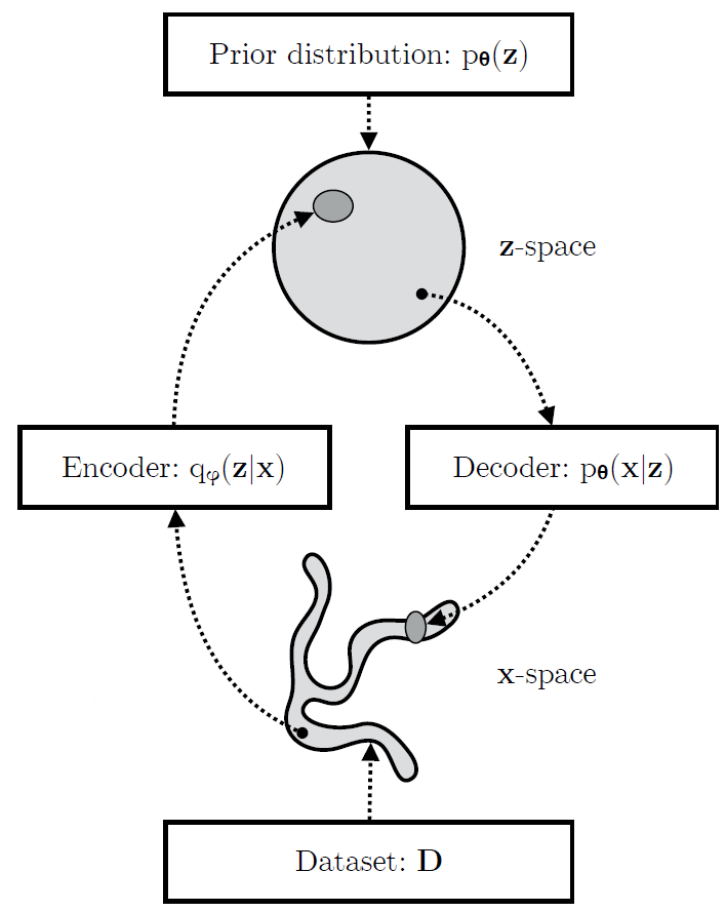
\includegraphics[scale=0.55]{vae.png}
\end{figure}

\subsection{Generative Adversarial Networks}
The goal of GANs is to model a data distribution with a generator. You can do that by forcing the generated samples to fit the data distribution by jointly training the discriminator, which tries to distinguish the generated samples from the target distribution. Generator maps from samples of a base distribution to samples of a target distribution and tries to fool the discriminator.\\
While training you alternatingly train the generator and discriminator in an unsupervised fashion.\\

Major problems are:
\begin{itemize}
    \item Tricky training (due to alternation, must keep equilibrium)
    \item Mode collaps (generator may generate only a small subset of distribution)
\end{itemize}

\newpage

\b{Style GANs\\[.5em]}
Style GANs try to control the image generation by a condition z (e.g. predefined style). The latent vector \f{z} is transformed into a vector \f{w} that is converted into a learned affine transformation (style).\\
This can for example be used to morph the styles of two different image sources.

\subsection{Diffusion Models}
The task is to learn to predict the small steps that turn a noisy image into a slightly less noisy image. The training data can be generated by iteratively adding Gaussian noise to the training images (self-supervised learning). Image generation starts from pure noise and iterates back towards a clean image.\\

\b{Conditioning the Diffusion Process\\[0.5em]}
Instead of modeling the unconditional mapping, the network (U-Net like) must take a condition \f{y} and produce the reverse noise based on that condition: \f{\nabla_x\log p(x|y)}. Via Bayes' rule, we get:
\cf{
    \nabla_x \log p(x|y) = \nabla_x \log p(y|x) + \nabla_x \log p(x)
}
which translates to:
\cf{
    \text{conditional diffusion step} = \text{predictive distr. (e.g. classifier)} + \text{unconditional diffusion step}.
}
The nice thing here is that this conditional can be added post-hoc, meaning after model training. However, classifiers are not made for noisy images, so the gradient is often bad.\\
Alternatively, we can of course directly train a conditional diffusion model. In practice, the condition is sometimes dropped during training so that the model also learns the unconditional distribution.\\ \f{\to} This leads to much better results.\\

\b{Note:} We cannot just use an unconditional model and adapt it, but require training on the target distribution of conditioned data. BUT: The unconditional model can be used as initialization.

\newpage

\subsection{Final Remarks}
\begin{itemize}
    \item Direct decoder models are notprobabilistic, but most straightforward
    \item GANs, VAEs, and diffusion modelshave probabilistic components
    \item To control what is being generated, some conditioning is needed. Typically this is handled by training with an appropriate conditional distribution.
\end{itemize}
\vspace{2cm}
\begin{figure}[h!]
    \centering
    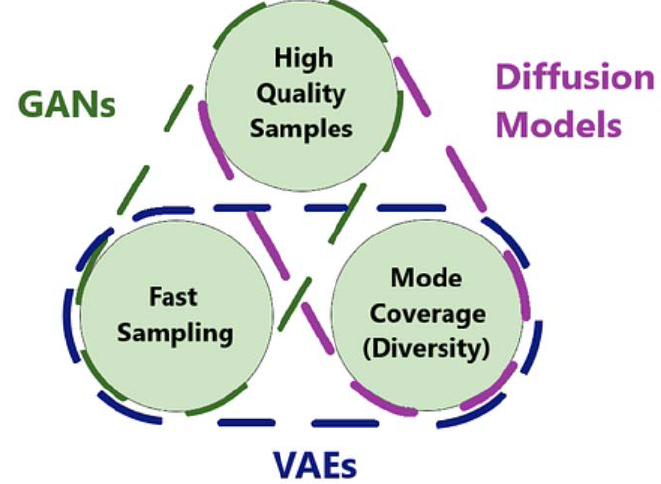
\includegraphics[width=0.5\textwidth]{gen.png}
\end{figure}







\newpage
\section{Next Generation Deep Learning}

\subsection{Supervised Learning}
Most deep learning follows the supervised paradigm, which is a mapping task learned from input-output pairs.\\

The harder the task the more training data is required.\\

What makes a task hard? \f{\to} Dimensionality and complexity of the data

\subsection{Unsupervised Learning}
Motivation: there are (almost) arbitrary amounts of unlabeled data. Ideally, we could learn from these. This is called unsupervised or self-supervised learning.\\

Self-supervised pretraining is competitive with supervised pretrainingon the ImageNet classification task.\\

Problem: If the output is undefined, the network can learn anything. What is a good training objective?\\

Traditional approach: Reconstruct the output (autoencoder) and compute reconstruction error.\\

\b{(Masked) Autoencoders\\[0.5em]}
Autoencoders typically do not learn semantically meaningful features since the reconstruction loss cares about pixel details, not semantics.\\

\b{Masking} some input image patches forces the encoder to care more about semantics as new content must be generated by the decoder based on the encoded context.\\

\b{Note:} Bottleneck acts as dimensionality reduction.\\

\b{Exemplar CNN\\[0.5em]}
An alternative approach to Masked Autoencoders. Involves training a network to discriminate surrogate classes. Each class is defined by a random seed patch and its transformed versions(translation, rotation, scaling, color, contrast, brightness, blur). This can also be seen as a extreme version of data augmentation. The transformations define invariance properties of the features to be learned.\\

\b{Contrastive Learning\\[0.5em]}
The principle of surrogate classes can be generalized to a contrastive loss to learn a feature embedding. \\

Main idea: for a sample define another positive sample that should be close in embedding space, and multiple negative samples that should be far. Positives and negatives can often be defined without supervision (self-supervised).\\

See DL summary for more!\\
\newpage

\b{DINO\\[0.5em]}
DINO uses a loss similar to a contrastive loss but with only positive samples: maximizing the similarity of the output distribution (cross-entropy).\\

To avoid collapse without negative samples, the teacher is updated only via the exponential moving average of the student network.\\

Transformed versions of an image are created (also) by local cropping operations. Only the teacher sees the global view.\\

\b{Other Self-Supervised Tasks\\[0.5em]}
Jigsaw-Puzzles, temporal order prediction

\subsection{Semi-Supervised Learning}
The goal is to combine the best of both worlds of supervised and unsupervised learning: exploit unlabeled data to require fewer labeled samples.\\

\b{Note:} Semi-supervised learning only works if the process that generates y from x is not independent of p(x).\\

\b{Student-Teacher Training\\[0.5em]}
The student is trained on labeled data while the teacher is the time-accumulated model of student models (EMA). The teacher provides an additional consistency loss on unlabeled data (pseudo-labels).\\

\b{Unsupervised Data Augmentation\\[0.5em]}
Label consistency over transformed inputs is used as an additional loss. This can also be seen as a regularizer.\\

\b{Noisy Student\\[0.5em]}
Train teacher model with labeled data \f{\to} Get pseudo-labels on unlabeled data \f{\to} Train equal or larger student with combined data and noise (augmentations) \f{\to} Make the student the new teacher \f{\to} Repeat the process\\

\b{Segmentation with GAN\\[0.5em]}
A segmentation network acts as the generator. It is trained partially on labeled samples using a regular cross-entropy loss. On unlabeled samples, the discriminator score acts as loss (the discriminator gets the input image and the segmentation as input).\\
Here the GAN learns a conditional distribution (input image as condition).


\subsection{Vision-Language Models}
Idea: Learn joint embedding spaces for vision and language. This provides visual grounding for text models and weak supervision for vision models.\\

If this is done with web-scale datasets, the resulting models are called \b{Foundation Model}. These give rise to a whole new set of applications: Multi-modal retrieval (find images via text, or vice-versa), "zero-shot” classification, open vocabulary detection, text-conditioned image generation.
\newpage

\b{CLIP\\[.5em]}
CLIP makes use of the description which are often added to images on the internet to create a shared embedding space.
\begin{figure}[h!]
    \centering
    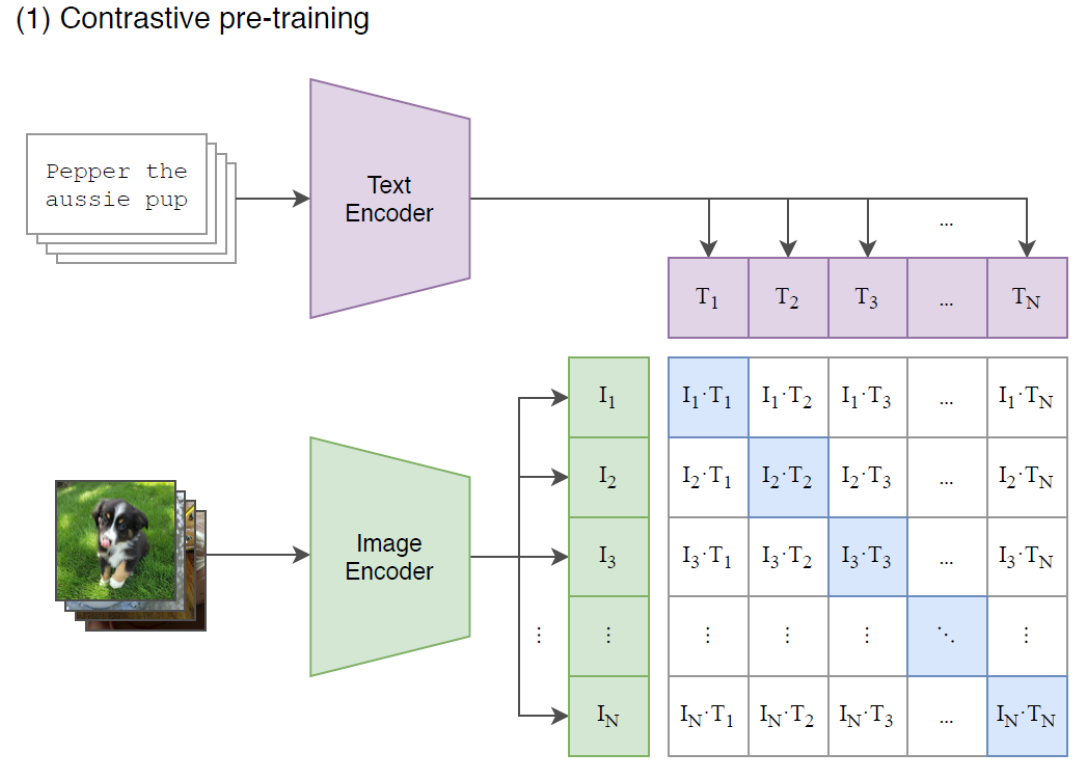
\includegraphics[width=.5\textwidth]{clip.png}
\end{figure}

\b{Distribution Shifts and Foundation Models\\[.5em]}
Most ML learning assumes that the test data is from the same distribution as the training data. Domain gap examples are:
\begin{itemize}
    \item synthetic vs. real data
    \item weather conditions, other backgrounds
    \item new camera with different resolution
\end{itemize}

If a domain gap exists, the source and target domain have to be adapted to fit each other (very tedious). As foundation models cover nearly all domains, they will never be out of distribution. In other words, one can avoid domain adaption by using foundation models (as backbone) for various domains/tasks.\\

To cover all domains, we need very large datasets (web-scale). This amount of data can not be labeled, so foundation models have to rely on self-supervised learning. To produce outputs for a wide variety of data and tasks we need a large model with enough capacity, which makes foundation models extremely compute intensive.\\

\b{Status quo for Foundation Models\\[.5em]}
The currently best working example are Language Models. They leverage the abundance of text available on the internet in combination with a good self-supervised task (next token prediction). The downstream tasks are also very straightforward.\\

Computer Vision is mainly covered by image-language models, as image-language acts as noisy labeling. Note that resource requirements are even larger.


\end{document}
